% Settings for the default beamer theme
\documentclass[english, aspectratio=169]{beamer}
\usepackage[T1]{fontenc}
\usepackage[utf8]{inputenc}
\usepackage{tabularx}
\usepackage{listings}
\usepackage{babel}
\usepackage[ruled,vlined]{algorithm2e}
\SetAlgorithmName{Algoritmus}{algoritmus}{List of Algorithms}
\setcounter{secnumdepth}{3}
\setcounter{tocdepth}{3}

\makeatletter

\newcommand\makebeamertitle{\frame{\maketitle}}

% (ERT) argument for the TOC
\AtBeginDocument{%
  \let\origtableofcontents=\tableofcontents
  \def\tableofcontents{\@ifnextchar[{\origtableofcontents}{\gobbletableofcontents}}
  \def\gobbletableofcontents#1{\origtableofcontents}
}

% Theme settings
\usetheme{Frankfurt}
\usecolortheme{default}
\usefonttheme[onlymath]{serif}

% Template settings
\setbeamertemplate{navigation symbols}{}
\setbeamertemplate{blocks}[rounded][shadow=false]
\setbeamertemplate{title page}[default][colsep=-4bp, rounded=true, shadow=false]
\makeatother

% Define a custom darker red color
\definecolor{DarkerRed}{RGB}{139,0,0} % Adjust the RGB values as needed

% Use the newly defined color in Beamer theme elements
\setbeamercolor{structure}{fg=DarkerRed} % Changes basic structural elements to Darker Red
\setbeamercolor{title in head/foot}{bg=DarkerRed} % Changes the title in header/footer to Darker Red

\lstset{
  language=Python,                 % choose the language of the code
  basicstyle=\ttfamily\small,      % the size of the fonts used for the code
  keywordstyle=\color{blue},       % keyword style
  stringstyle=\color{red},         % string literal style
  commentstyle=\color{green},      % comment style
  morecomment=[l][\color{magenta}]{\#},
  tabsize=4
}

\begin{document}

% Title page
\section{Bevezetés}
\title[]{Üzleti Elemzések Módszertana}
\subtitle{11. Előadás: Megerősítéses tanulás}
\author[Kuknyó Dániel]{Kuknyó Dániel\\Budapesti Gazdasági Egyetem}
\date{2023/24\\2.félév}
\makebeamertitle

% Table of contents slide
\begin{frame}
\tableofcontents{}
\end{frame}

% Table of contents of the current section
\begin{frame}
\tableofcontents[currentsection]
\end{frame}

\begin{frame}{A gépi tanulás fajtái}
A gépi tanulás 3 fő irányzata:
\begin{itemize}
	\item Felügyelt tanulás
	\item Felügyelet nélküli tanulás
	\item Megerősítéses tanulás
\end{itemize}
\begin{center}
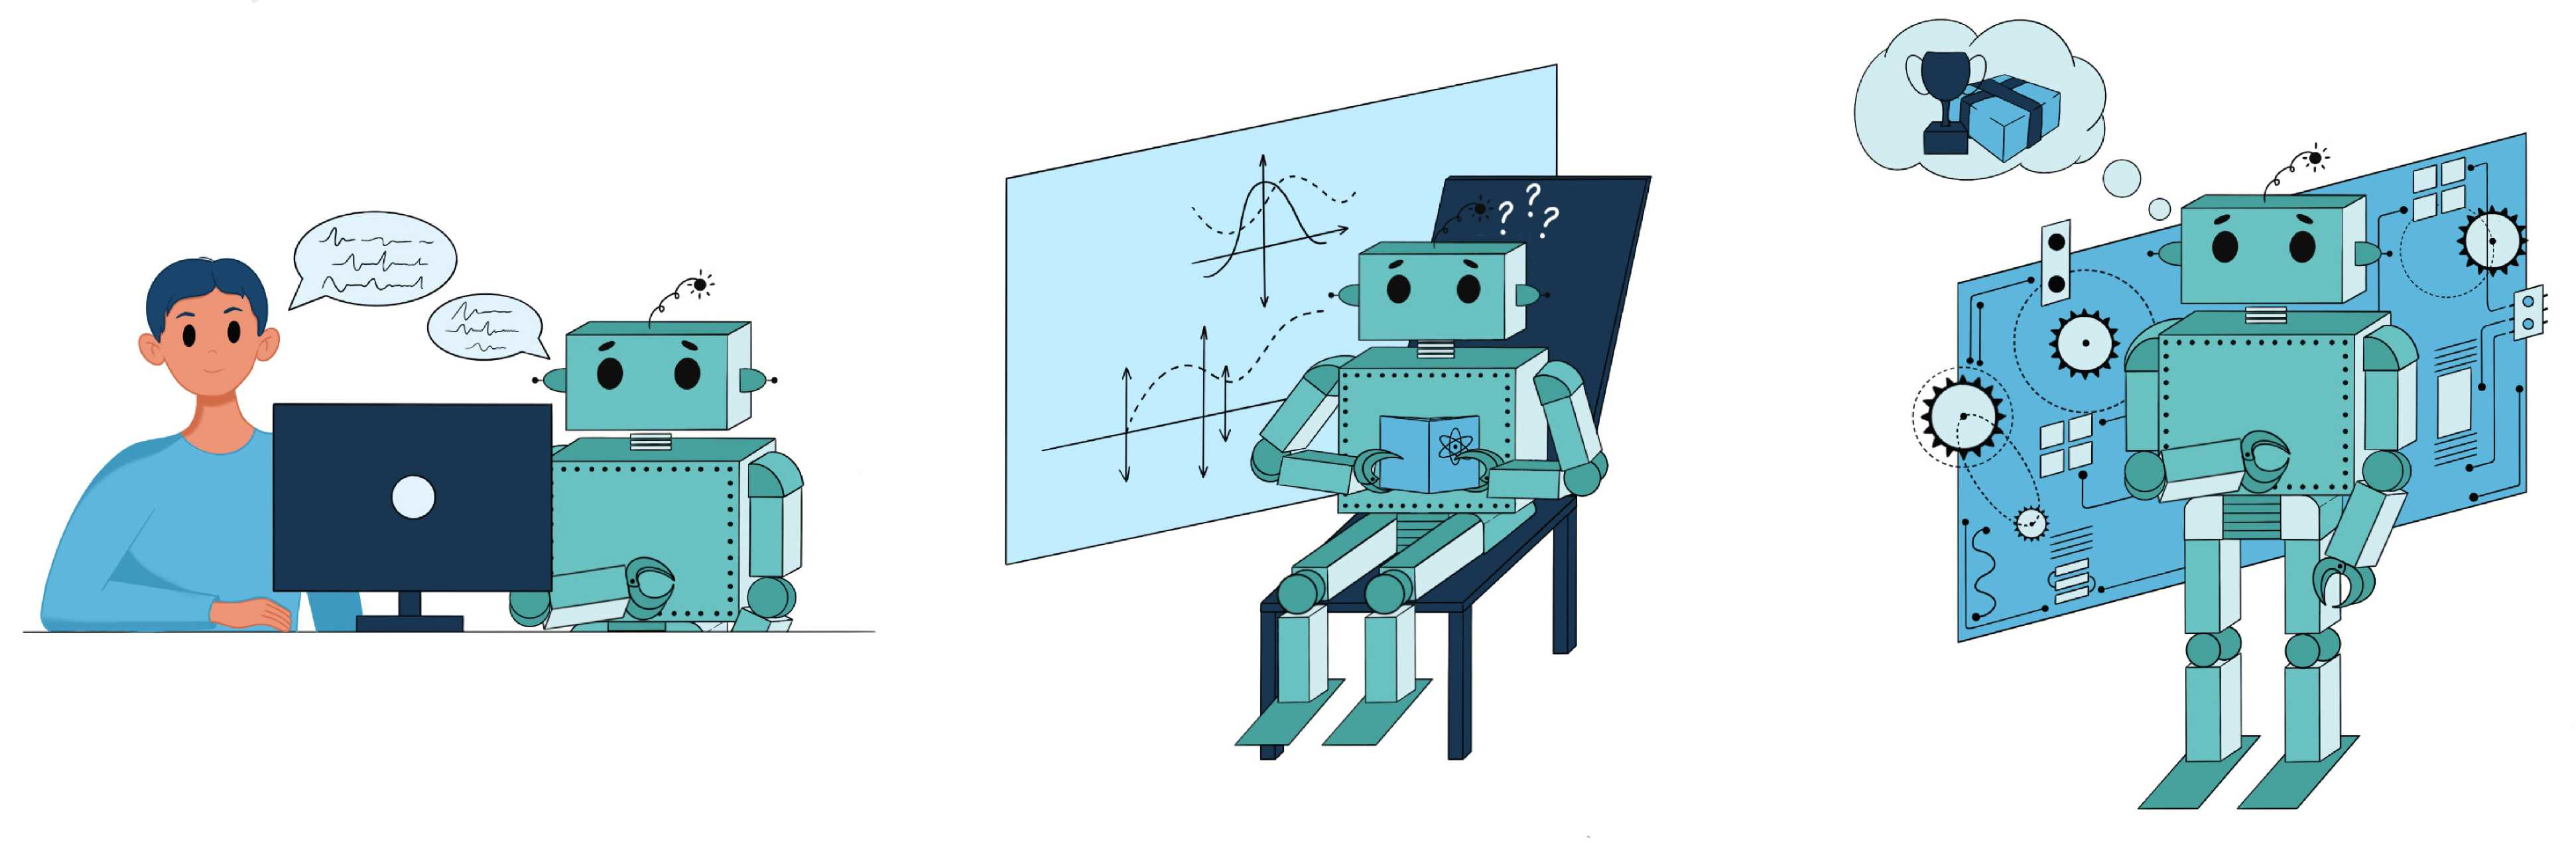
\includegraphics[width=12cm, height=7cm, keepaspectratio]{images/reinforcement_1.png}
\end{center}
\end{frame}

\begin{frame}{Mikor alkalmazható a megerősítéses tanulás?}
\begin{columns}
\begin{column}{.5\textwidth}
Az RL olyan problémák esetén használatos, ahol\textbf{ az algoritmikus vagy hagyományos ML hozzáállás nem bizonyul megfelelőnek}, mert nem lehetséges tanító adatot gyűjteni vagy generálni.\par\smallskip
Például:
\begin{itemize}
	\item Robotok
	\item Autonóm vezetés
	\item Számítógépes játékok
\end{itemize}
\end{column}
\begin{column}{.5\textwidth}
\begin{center}
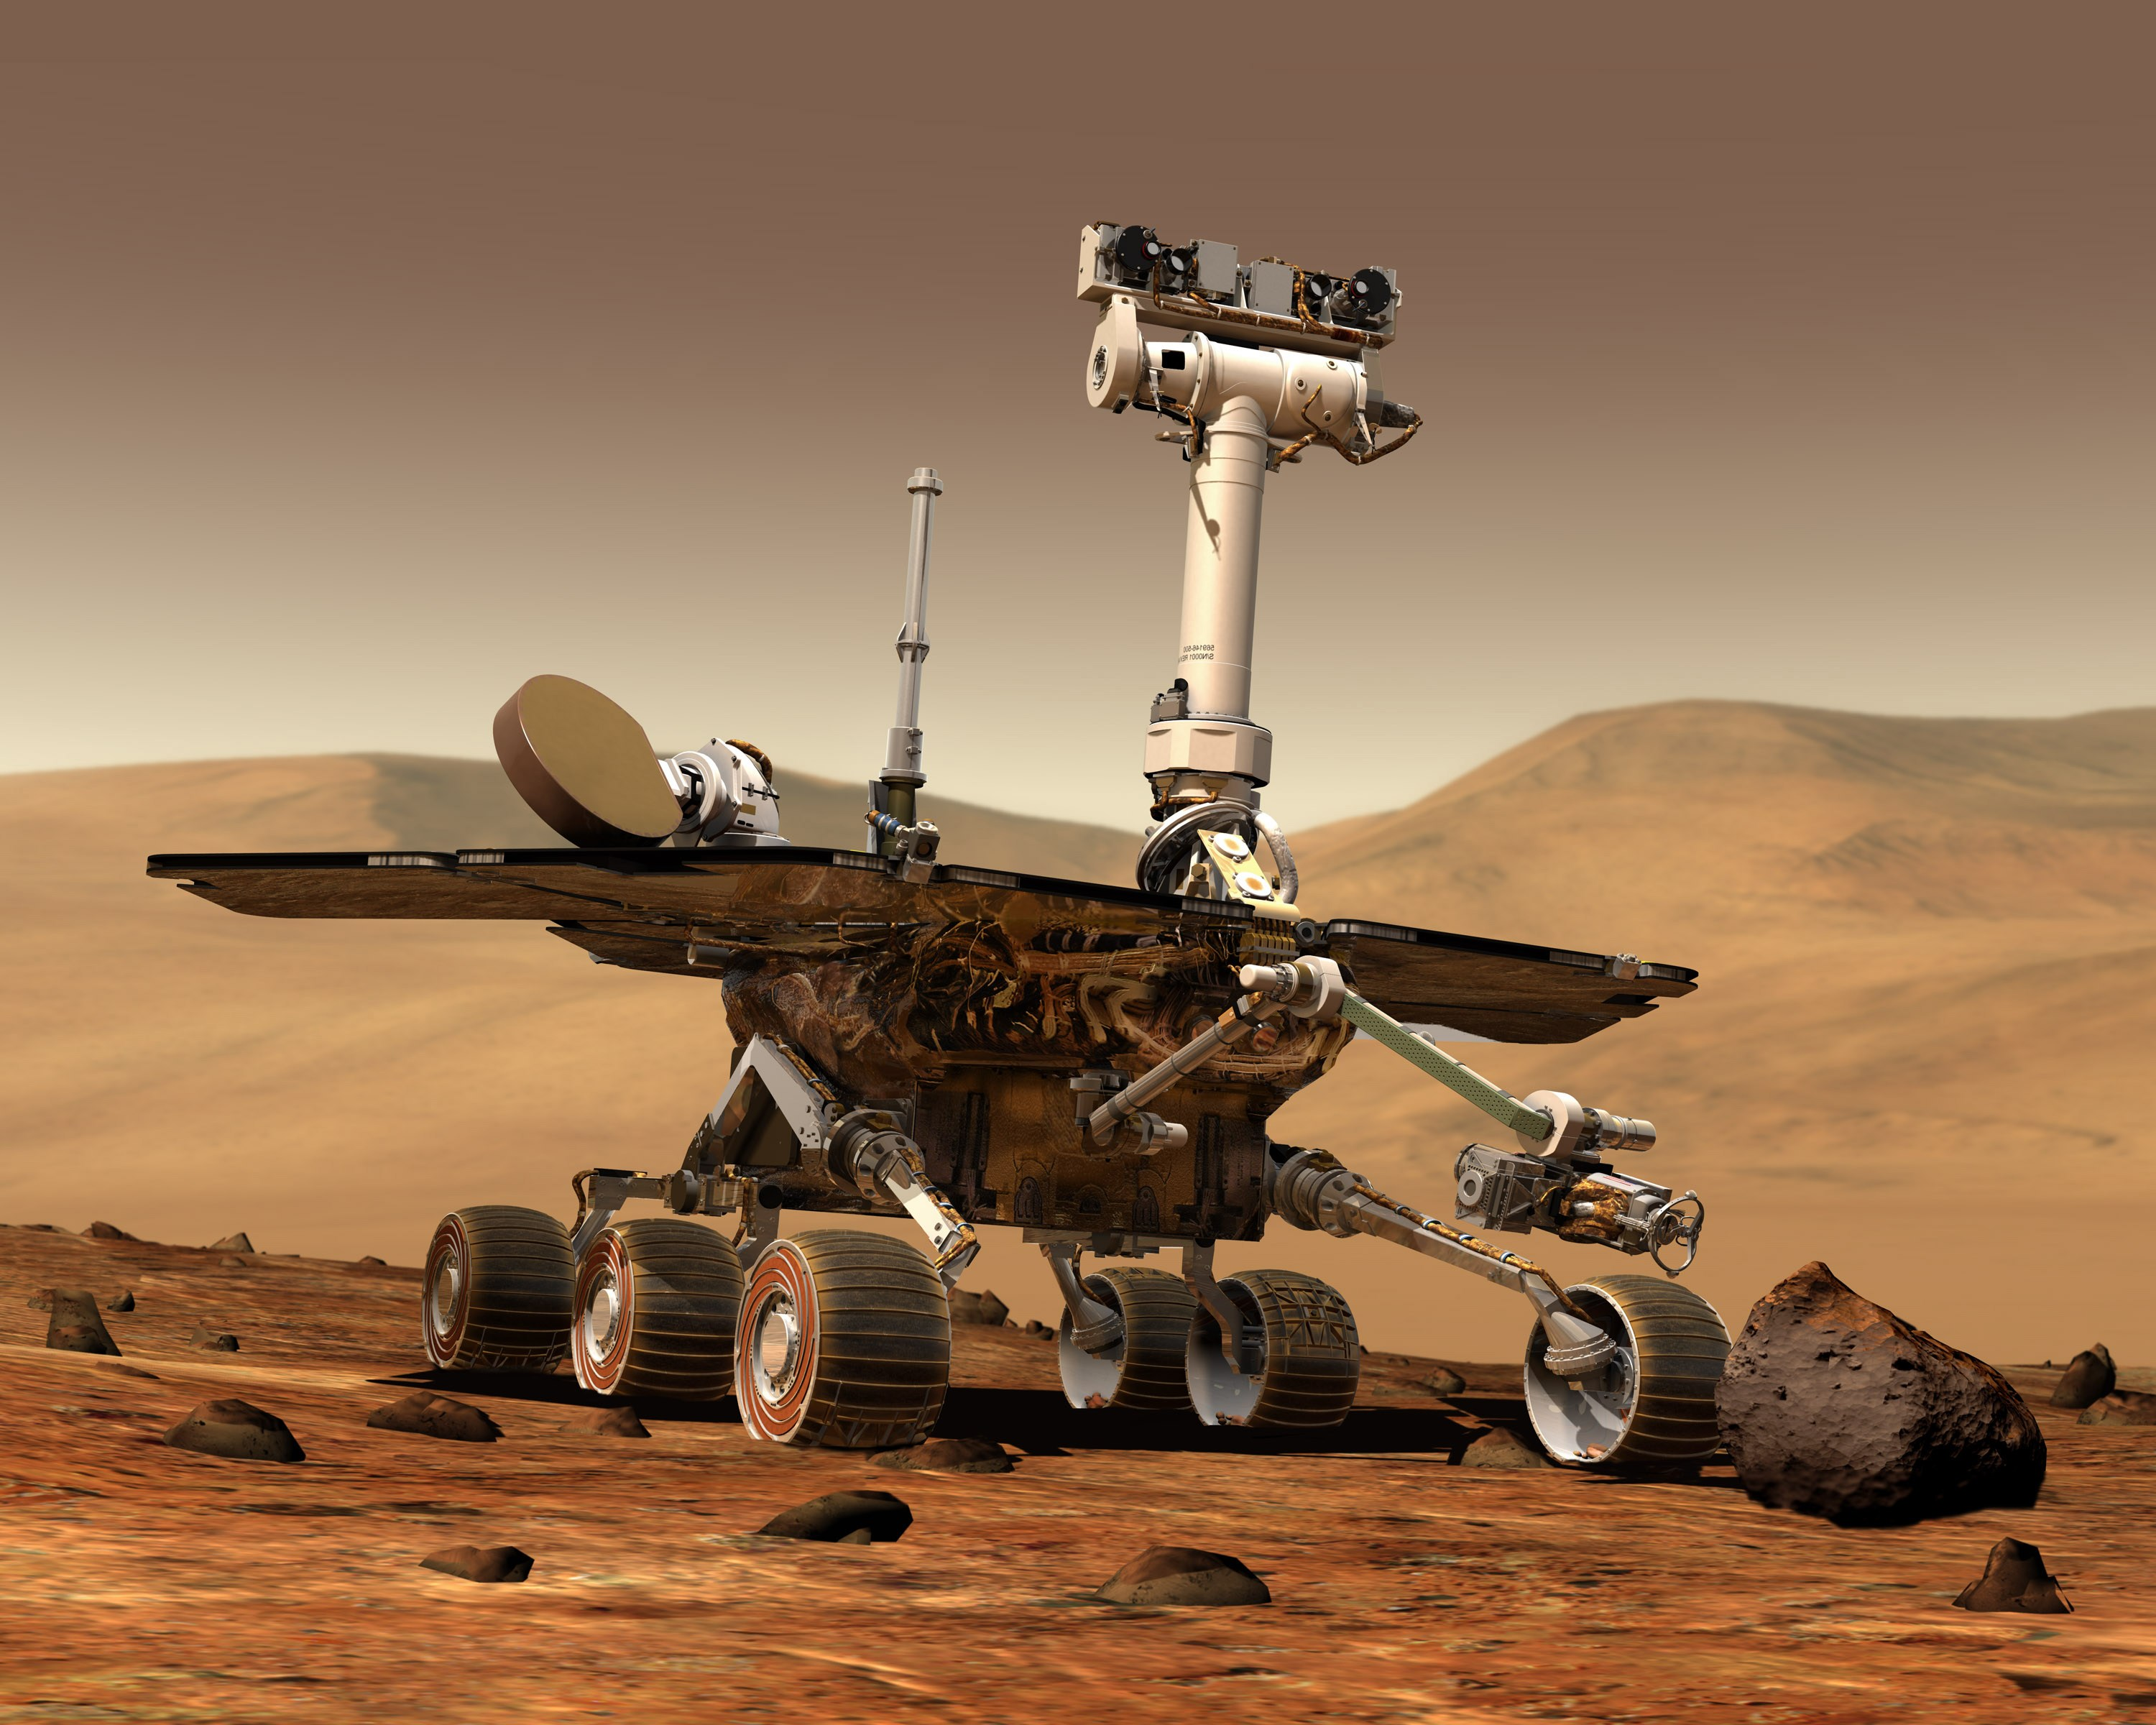
\includegraphics[width=3cm, height=2.5cm]{images/reinforcement_2.png}
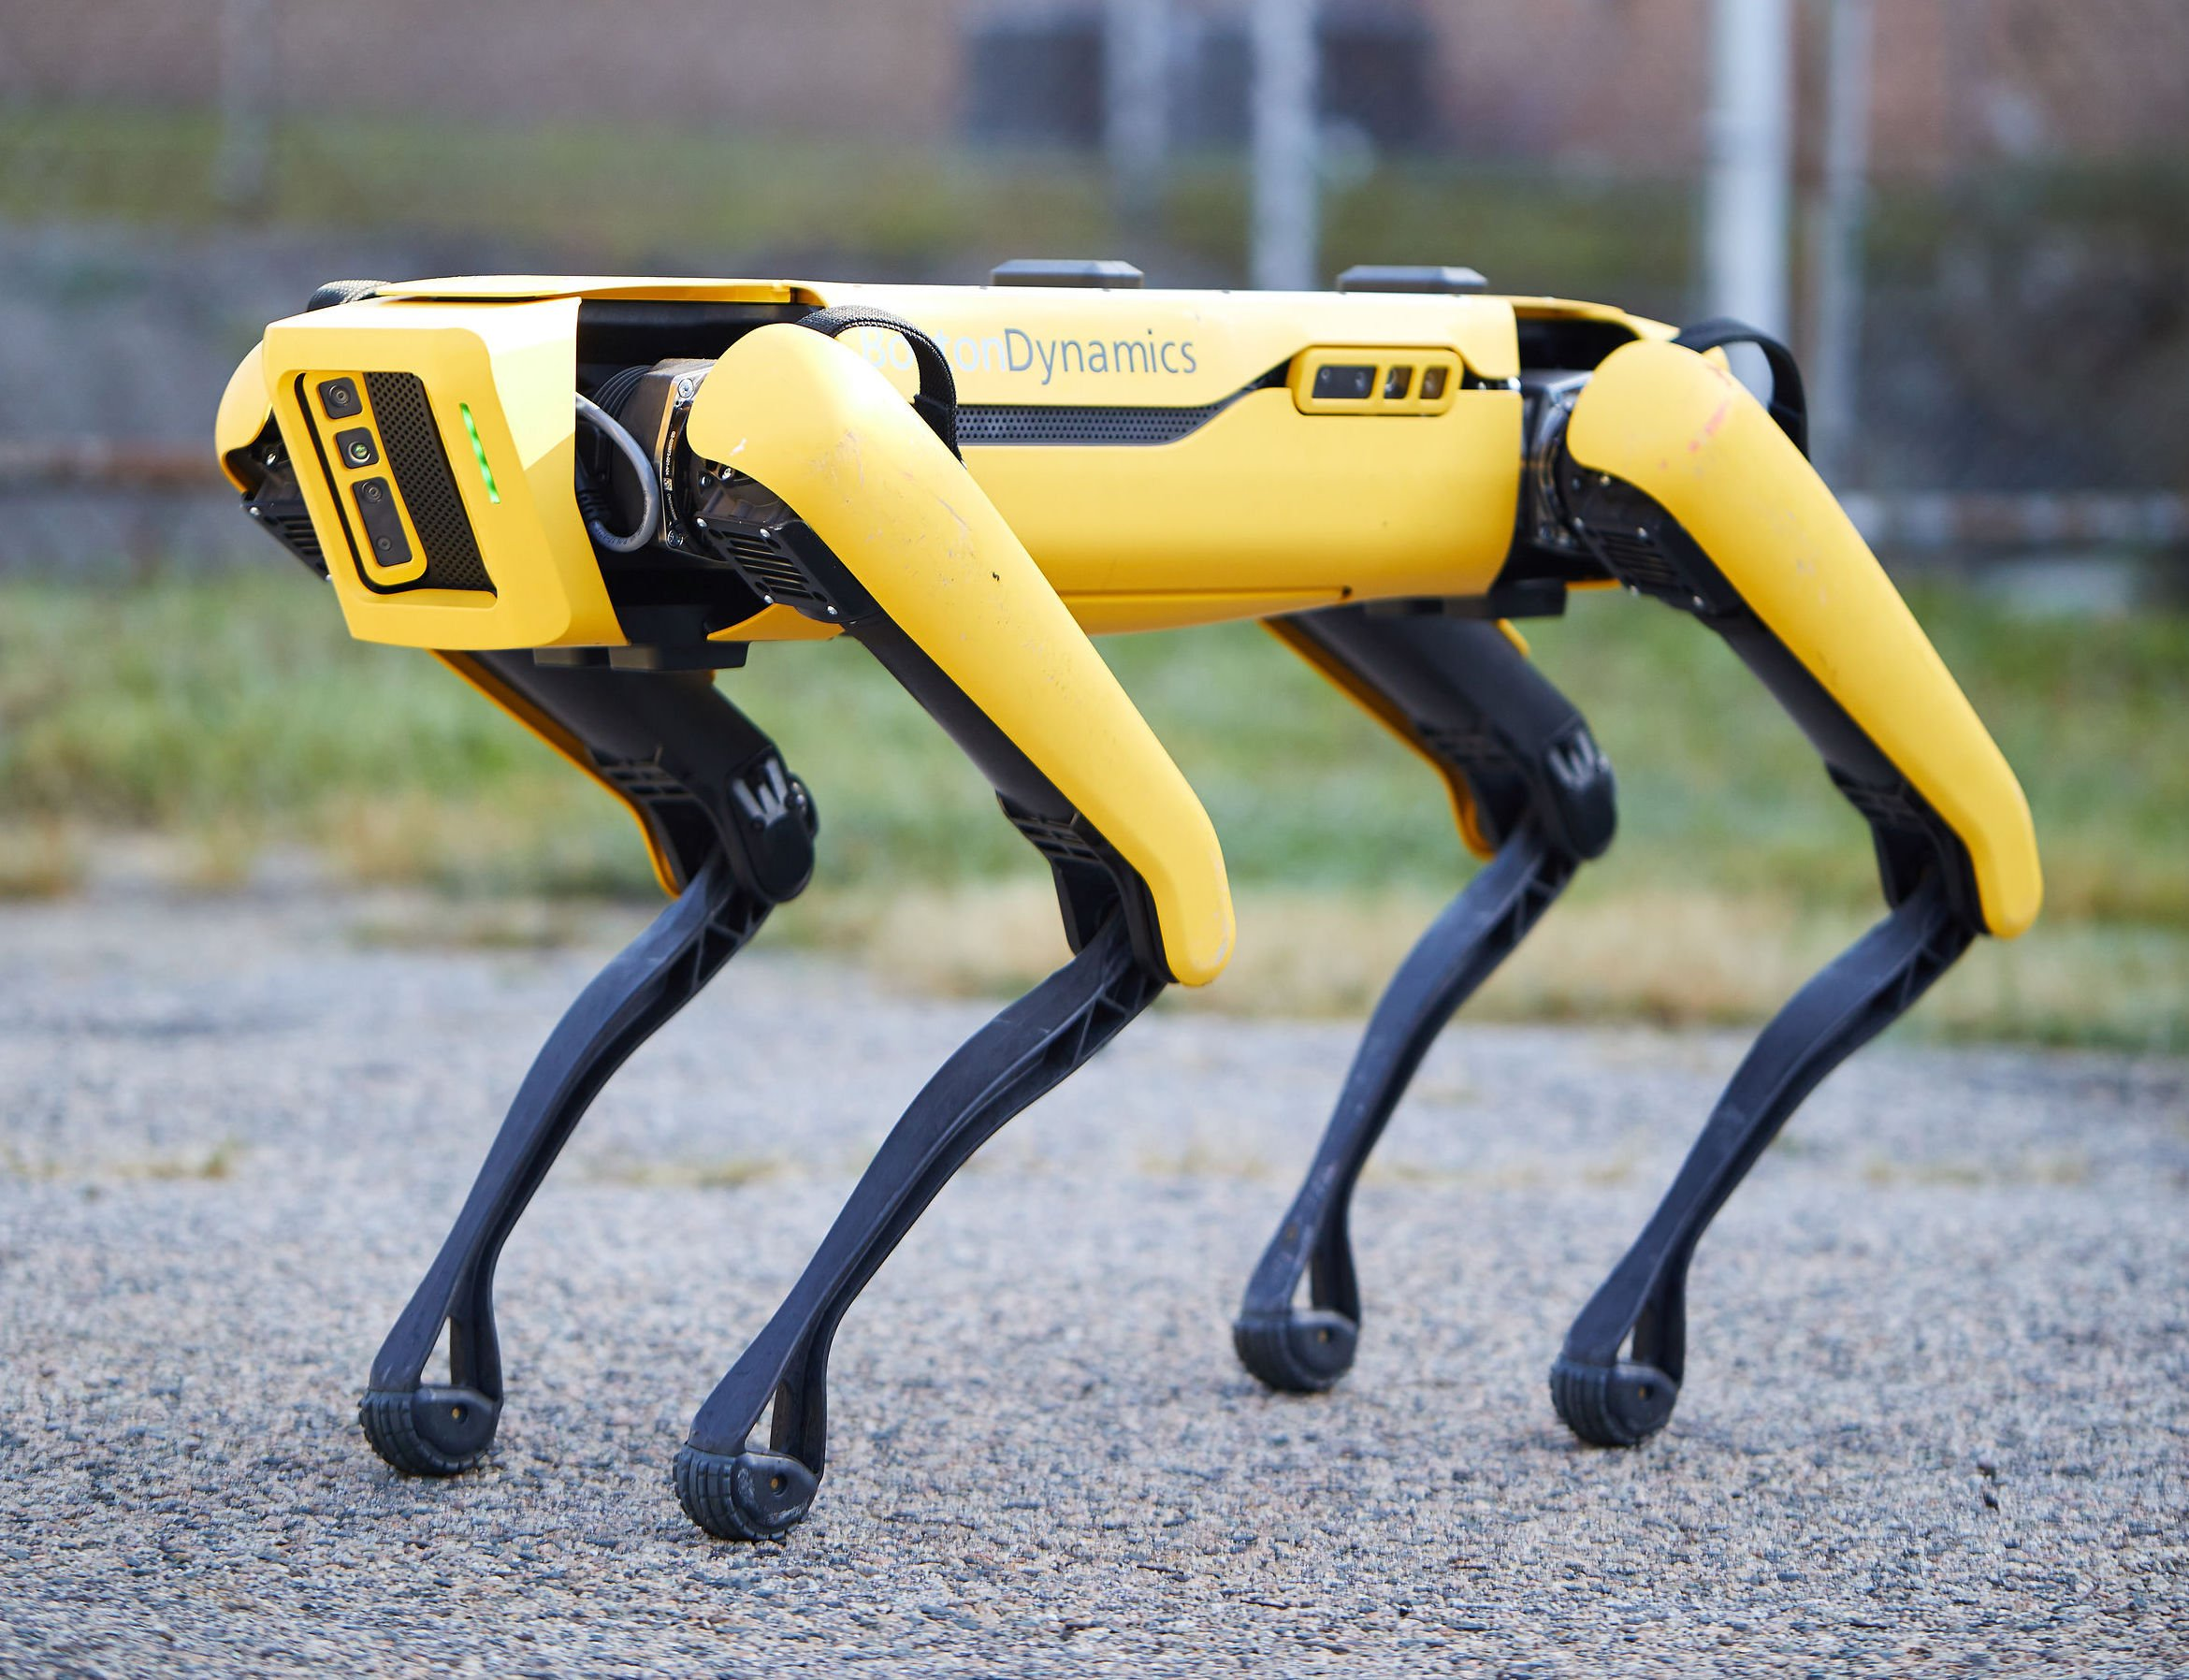
\includegraphics[width=3cm, height=2.5cm]{images/reinforcement_3.png}
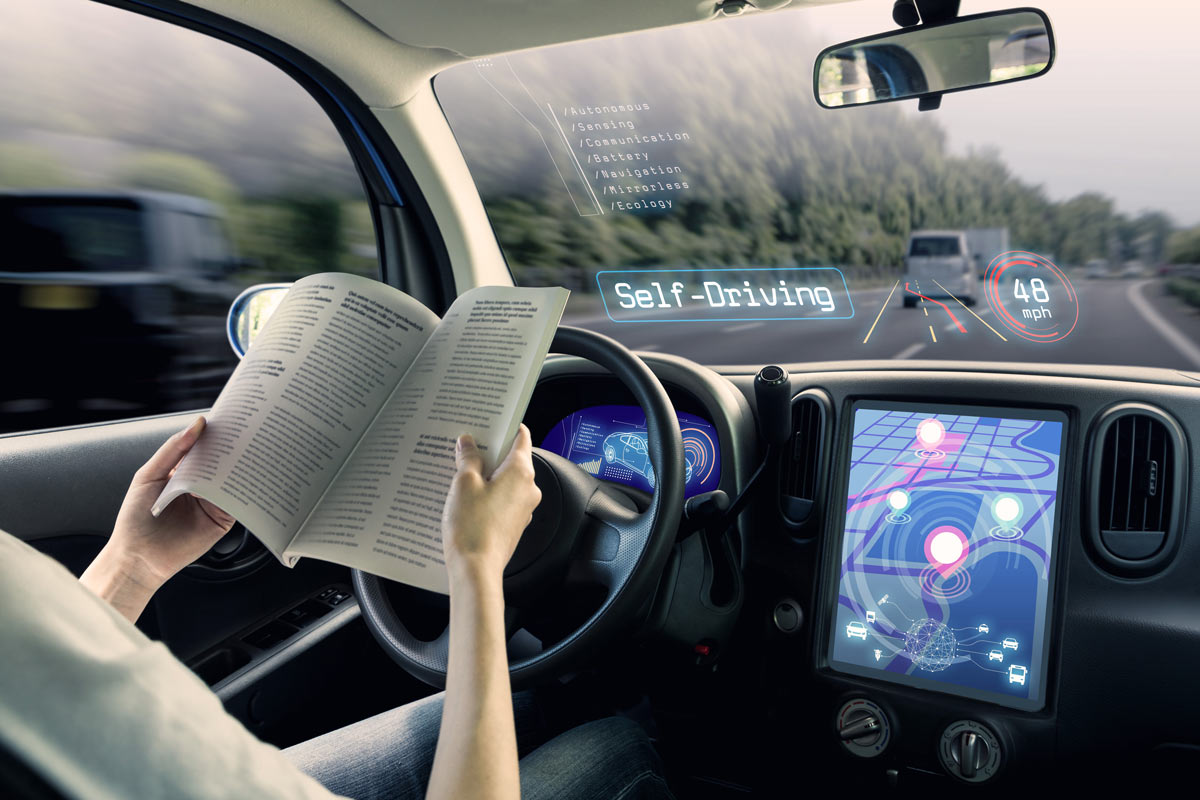
\includegraphics[width=3cm, height=2.5cm]{images/reinforcement_4.png}

\includegraphics[width=3cm, height=2.5cm]{images/reinforcement_5.png}
\end{center}
\end{column}
\end{columns}
\end{frame}

\begin{frame}{Felügyelt vagy megerősítéses tanulás?}
\begin{columns}
\begin{column}{.5\textwidth}
Adott például egy autóversenyző program. Ha felügyelt tanítás a választott hozzáállás, \textbf{szükség van egy adatbázisra, amely jellemzi az összes szituációt, és minden szituációhoz tartozóan az elvárt output értéket}.\par\medskip
A szituációknak le kell írnia a kocsi helyzetét, a környezet állapotát, a versenytársak helyzetét. Az elvárt outputnak olyan halmazból kell kikerülnie, mint gáz, jobb, bal, fék és ezek kombinációi.
\end{column}
\begin{column}{.5\textwidth}
\begin{center}
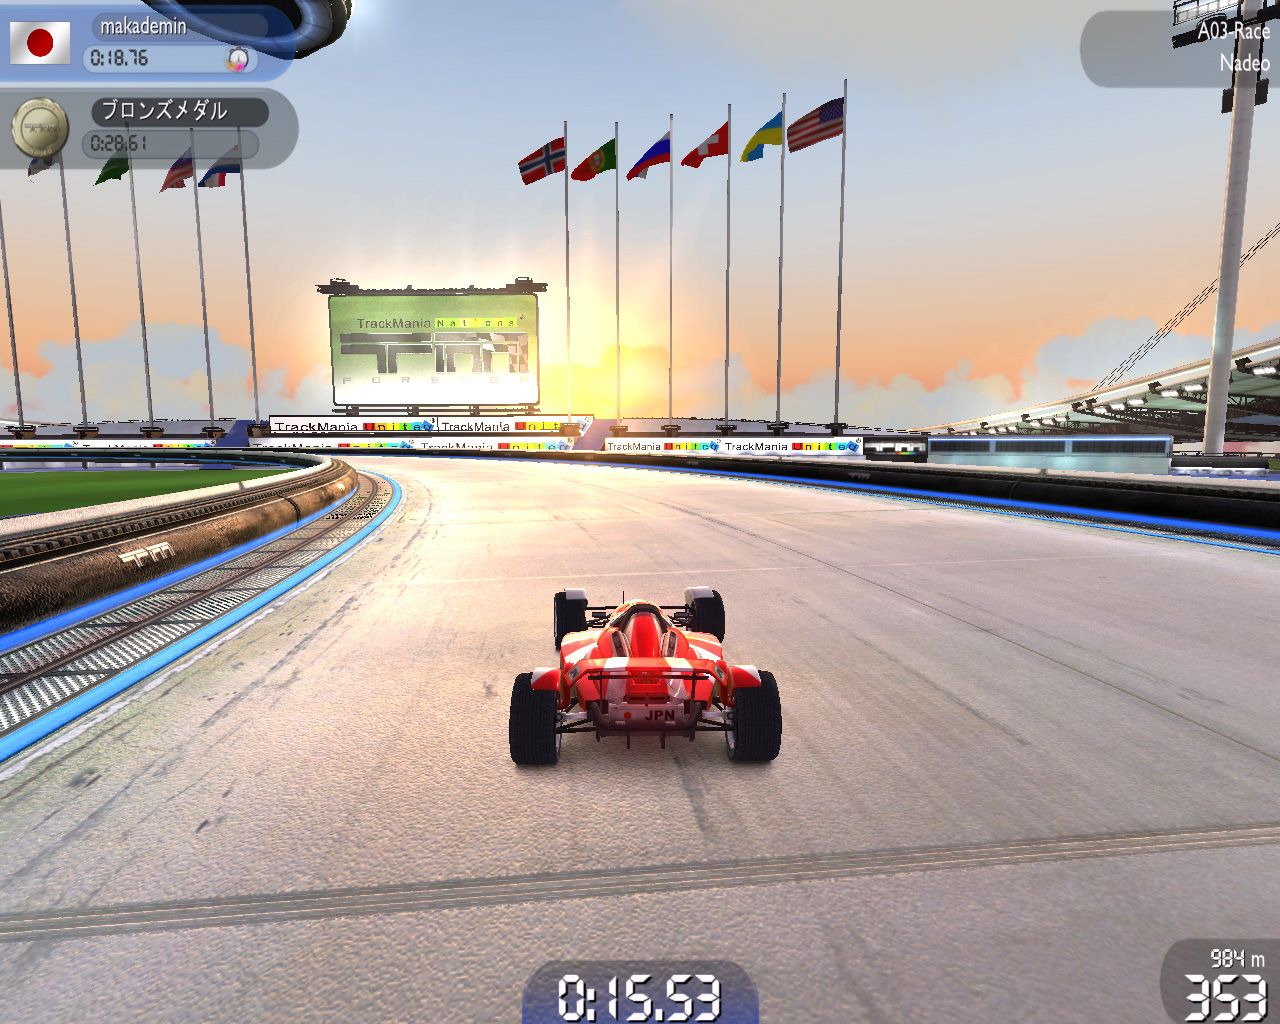
\includegraphics[width=6cm, height=7cm, keepaspectratio]{images/reinforcement_6.png}
\end{center}
\end{column}
\end{columns}
\end{frame}

\begin{frame}{Visszajelzések a megerősítéses tanulásban}
\begin{columns}
\begin{column}{.5\textwidth}
A két szemléletmód abban különbözik, hogy a felügyelő milyen visszajelzéseket ad a tanulónak.\par\medskip
\only<1>{\textbf{A felügyelt tanulásban teljes visszajelzésekről van szó, mert a válasz önmagában a  megoldás.}}
\only<2>{\textbf{A megerősítéses tanulásban viszont csak részlegesek a visszajelzések. A felügyelő válasza mindig csak a megoldás irányába vezet, nem önmagában a teljes jó megoldás.}}
\end{column}
\begin{column}{.5\textwidth}
\begin{center}
\includegraphics<1>[width=7cm, height=7cm, keepaspectratio]{graphs/reinforcement_1.png}
\includegraphics<2>[width=7cm, height=7cm, keepaspectratio]{graphs/reinforcement_2.png}
\end{center}
\end{column}
\end{columns}
\end{frame}

\begin{frame}{A megerősítéses tanulás komponensei}
\begin{columns}
\begin{column}{.3\textwidth}
\begin{center}
\only<1>{\begin{block}{Ügynök}
Az autonóm cselekvő, ami a feladat végrehajtására törekszik.
\end{block}}
\only<2>{\begin{block}{Környezet}
Egy fekete doboz, amely az ügynök cselekvéseinek helyszíne.
\end{block}}
\only<3>{\begin{block}{Idő}
RL folyamán az időlépések diszkrétek:\\
$t\in{1,2,3,...}$
\end{block}}
\only<4>{\begin{block}{Állapot}
Az ügynök megfigyelése a környezetre vonatkozóan. A környezetet leíró változók összessége.\\
Jelölés: $s\in{S}$, ahol $S$ az összes állapot halmaza.
\end{block}}
\only<5>{\begin{block}{Jutalom}
Az ügynök cselekvésének jóságát jelző skalár.\\
Jelölés: $r\in{\mathbb{R}}$
\end{block}}
\only<6>{\begin{block}{Cselekvés}
Az ügynök által végrehajtott művelet, ami a környezetet befolyásolja.\\
Jelölés: $a \in{A}$, ahol $A$ az összes cselekvés halmaza.
\end{block}}
\only<7>{\begin{block}{Politika}
Egy állapot $\rightarrow$ cselekvés leképezés. Az ügynök cselekvéseinek szabályait adja meg.\\
Jelölés:\\
\begin{itemize}
	\item Determinisztikus: $\pi\in{S\rightarrow}A$
	\item Sztochasztikus: $\pi\in{S\times}A\rightarrow [0,1]$\\
	Röviden: $\pi (s,a)$\\
	Vagy: $\pi (a|s)$
\end{itemize} 
\end{block}}
\end{center}
\end{column}
\begin{column}{.7\textwidth}
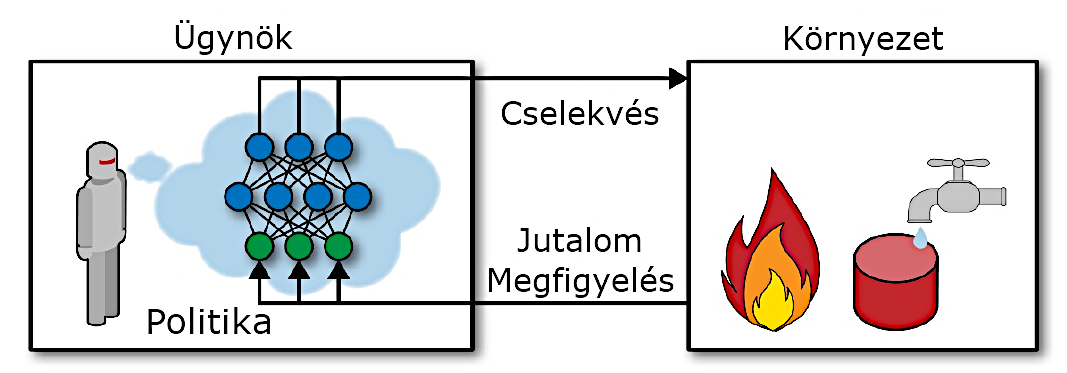
\includegraphics[width=10cm, keepaspectratio]{images/reinforcement_7.png}
\end{column}
\end{columns}
\end{frame}

\begin{frame}{Az ügynök}
\begin{columns}
\begin{column}{.5\textwidth}
A megerősítéses tanulásban egy ügynök \textbf{(cselekvő) megfigyeli a környezetet, és ezalapjáb cselekvéseket tesz a környezetben. A cselekvéseiért és a környezet változásáért jutalmat kap}.\par\smallskip
Az ügynök célja, hogy a jutalmakat hosszú távon maximalizálja. Az ügynök lehet:
\begin{itemize}
	\item A program, ami egy robotot irányít
	\item A program, ami PacMan-t irányítja
	\item Egy Go-t játszó program
	\item Lehet egy okos termosztát is
	\item Kereskedő a tőzsdén
\end{itemize}
\end{column}
\begin{column}{.5\textwidth}
\begin{center}
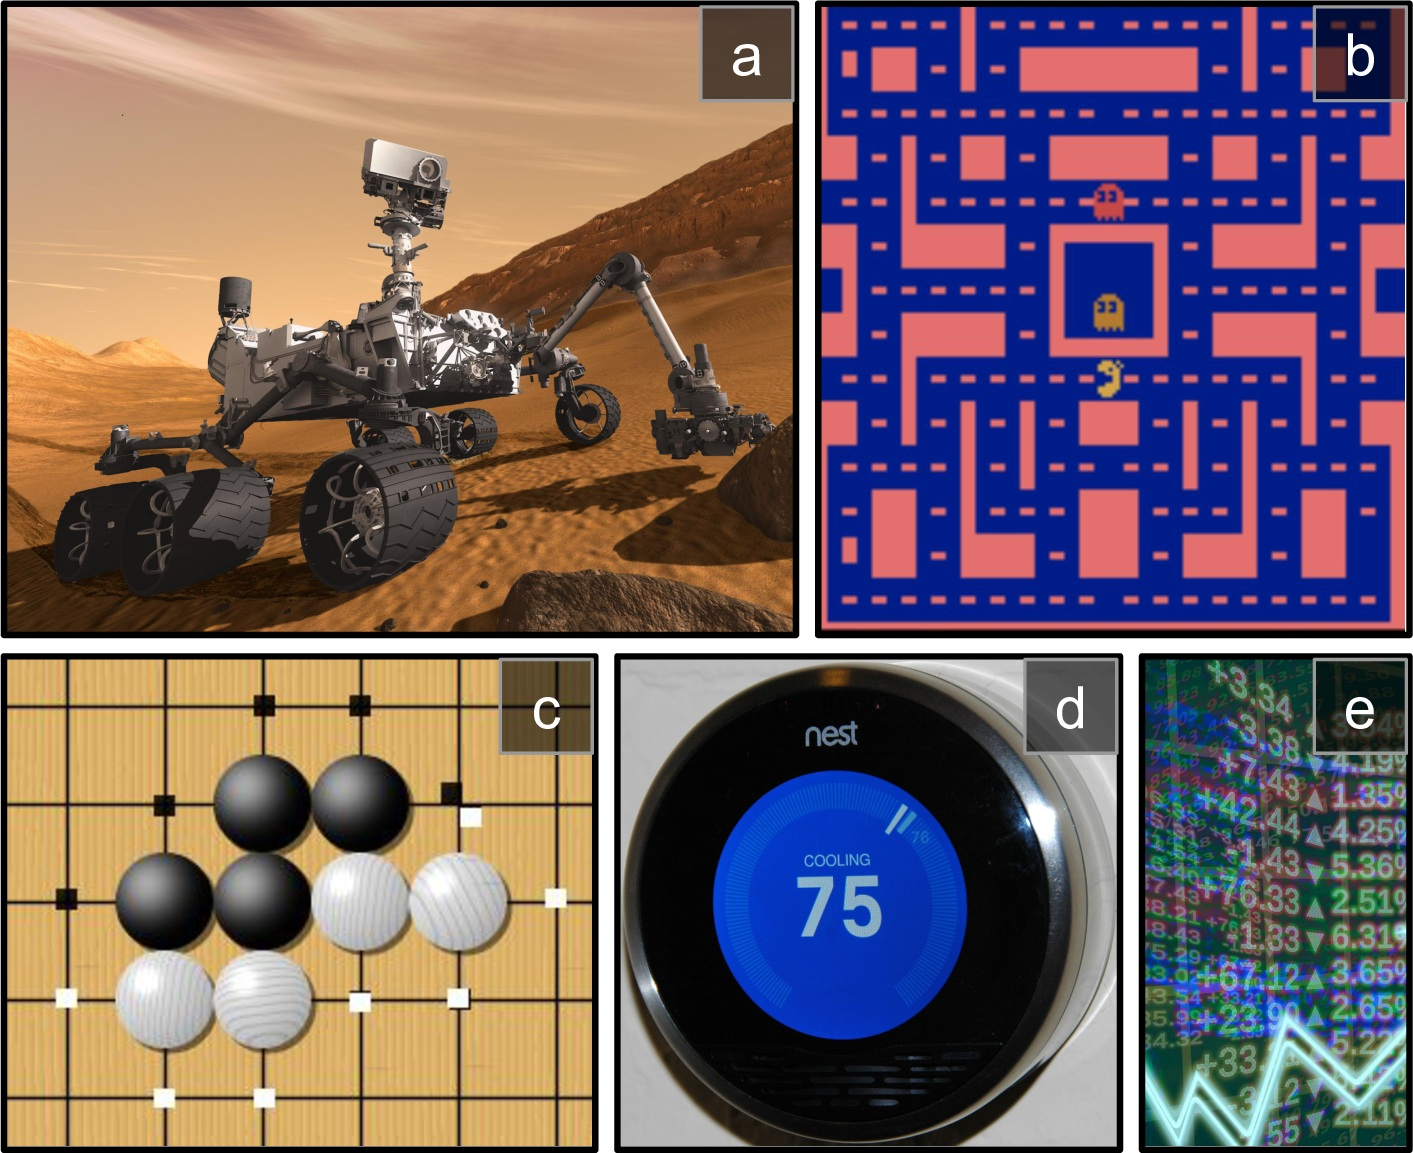
\includegraphics[width=7cm, height=7cm, keepaspectratio]{images/reinforcement_8.png}
\end{center}
\end{column}
\end{columns}
\end{frame}

\begin{frame}{Politika}
Az az algoritmus, ami az ügynököt irányítja. A politika által határozza meg az ügynök a cselekvéseit.\par\smallskip
\textbf{A politika egy modell, ami a környezetet leíró változókat fogadja bemenetként, és az outputja egy cselekvés a cselekvések választható halmazából.}
\begin{center}
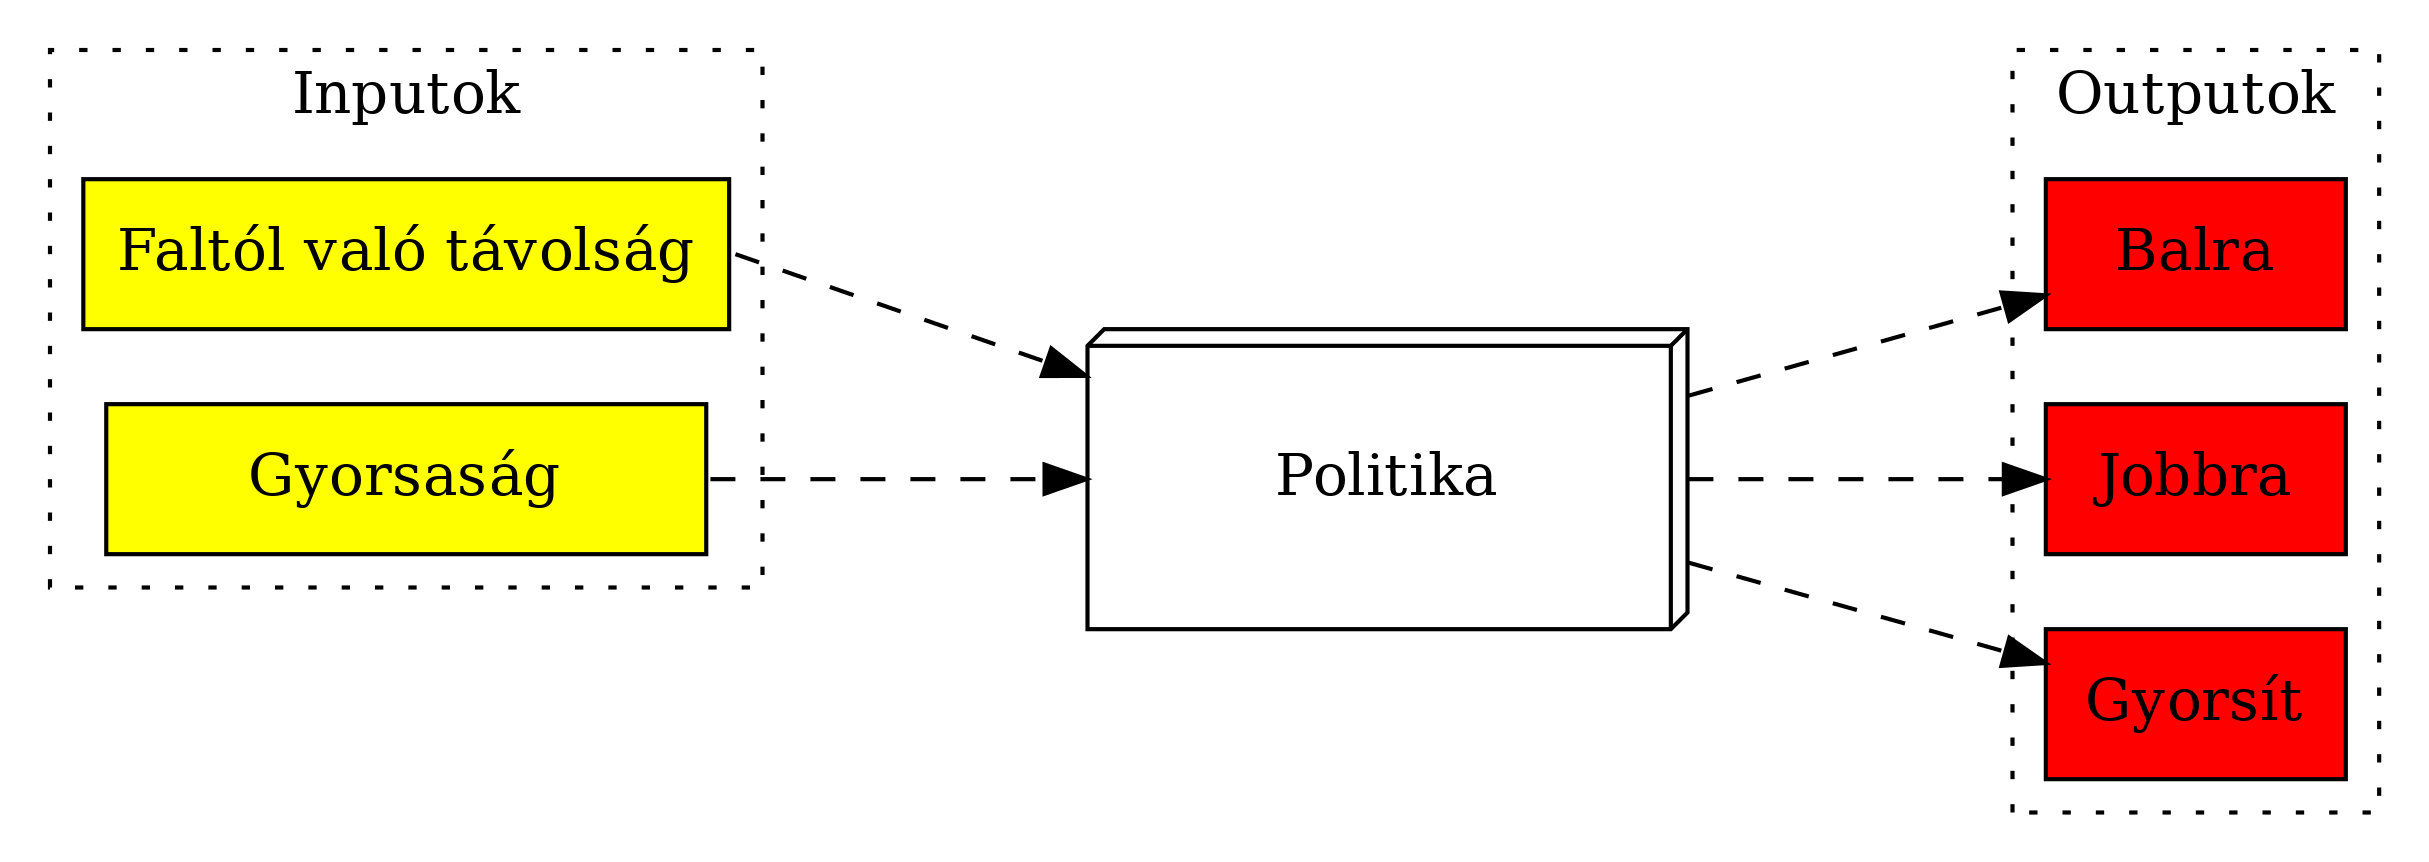
\includegraphics[width=12cm, height=7cm, keepaspectratio]{graphs/reinforcement_4.png}
\end{center}
\end{frame}

\begin{frame}{Interakció a környezettel}
\begin{columns}
\begin{column}{.5\textwidth}
\begin{itemize}
	\item Az ügynök és a környezet egymásra hatnak. Az ügynök cselekszik, ennek hatására a környezet megváltozik. Az ügynök megfigyeli a környezetet, majd ismét cselekszik:
	$s_1 \rightarrow a_1 \rightarrow s_2 \rightarrow a_2 \rightarrow ... \rightarrow s_t 			\rightarrow a_t$
	\item A jutalom azonnali, és cselekvés-állapot párosért jár: $R(s, a)$
	\item A környezet változását az átmeneti valószínűségek adják: $P(s'|s, a)$, ami $s'$ következő állapot valószínűsége $s$ állapotból, $a$ cselekvést követően. Ez a \textbf{környezet dinamikája}.
\end{itemize}
\end{column}
\begin{column}{.5\textwidth}
\begin{itemize}
	\item Az ügynök célja a lehető legmagasabb jutalom összegyűjtése hosszú távon: 
	\begin{block}{}
	\vspace{-0.2cm}
	\[
	E_{\pi}(r_{1}+r_{2}+r_{3}+...)\rightarrow{max}
	\]
	\end{block}		
\end{itemize}
\begin{center}
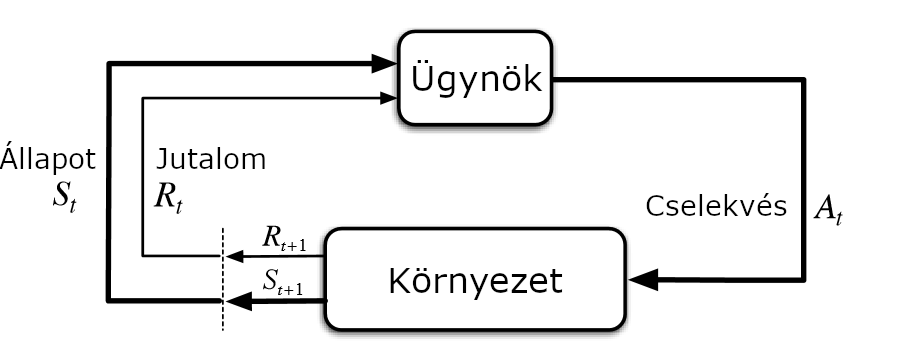
\includegraphics[width=7.5cm, keepaspectratio]{images/reinforcement_9.png}
\end{center}
\end{column}
\end{columns}
\end{frame}

\begin{frame}{Epizódok}
\begin{columns}
\begin{column}{.5\textwidth}
A megerősítéses tanulás egyetlen tanítási iterációja egy epizód. \textbf{Egy epizód addig tart, míg az ügynök el nem ér valamilyen vég/terminális állapotba.} A végállapot lehet: 
\begin{itemize}
	\item A cél teljesítése
	\item Teljes bukás / halál
	\item Időkeret lejárása
	\item Részfeladat teljesítése
	\item Jutalom összeg összegyűjtése
\end{itemize}
\end{column}
\begin{column}{.5\textwidth}
\begin{center}
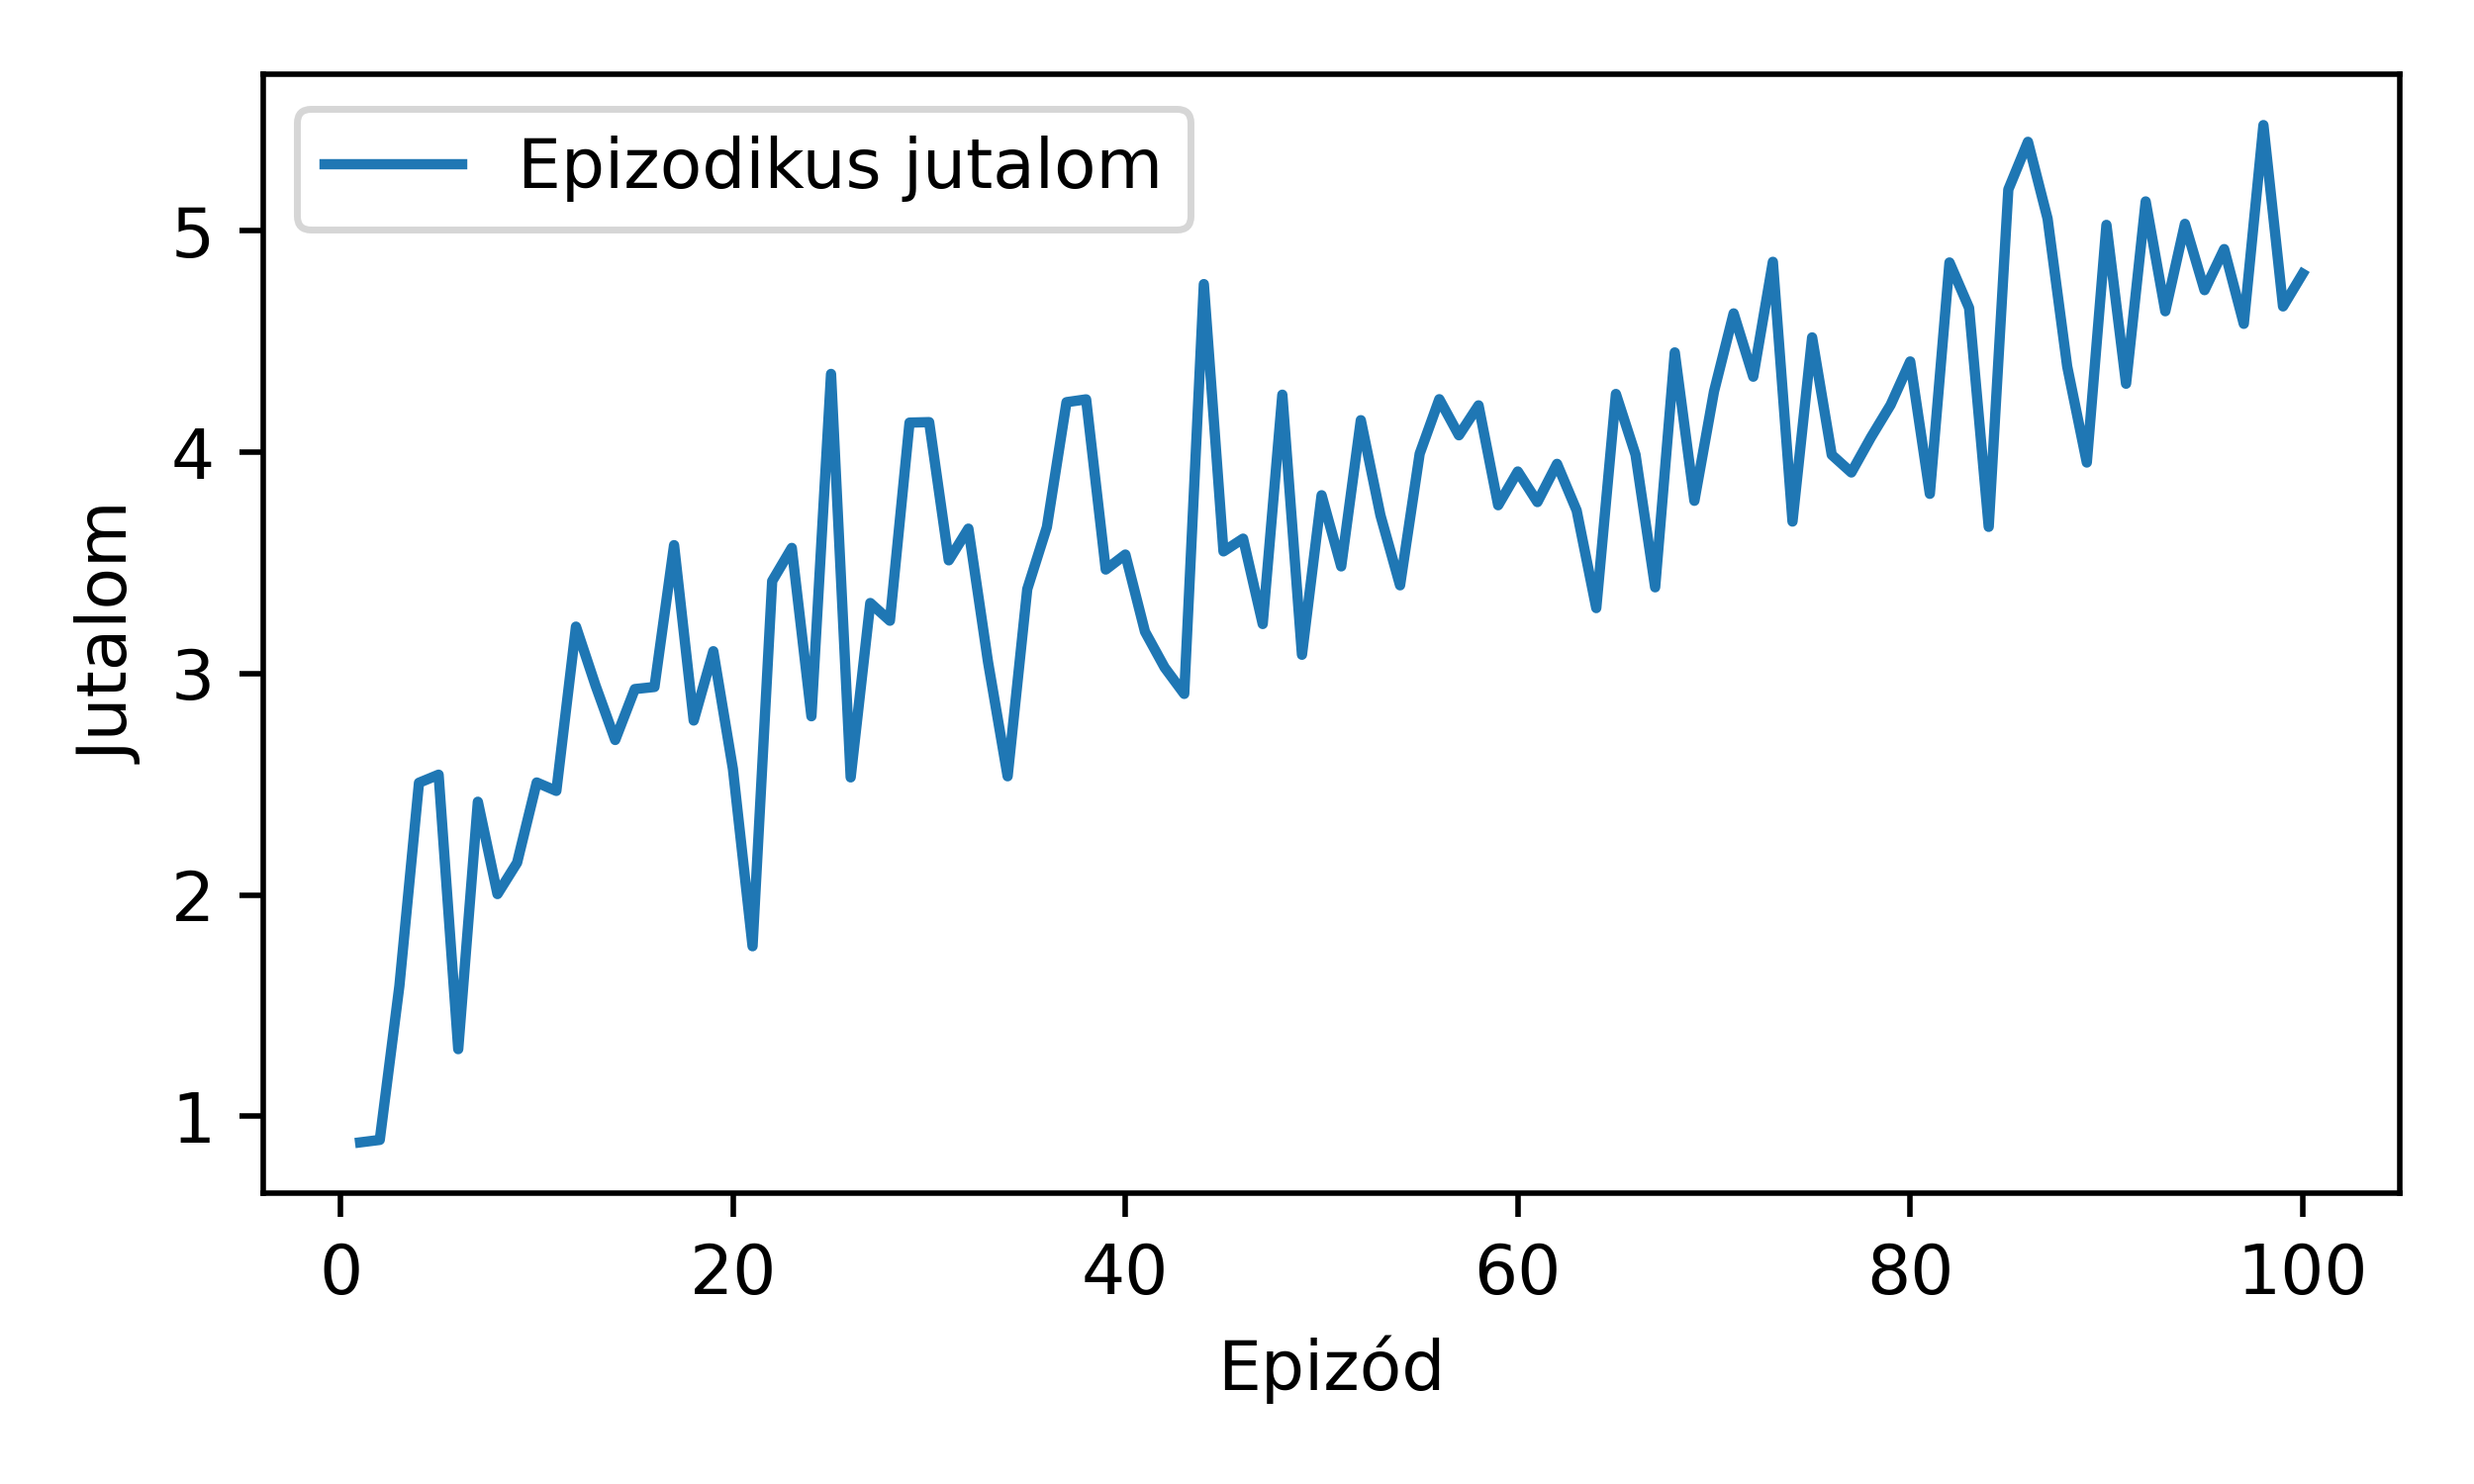
\includegraphics[width=7cm, height=7cm, keepaspectratio]{images/reinforcement_10.png}
\end{center}
\end{column}
\end{columns}
\end{frame}

\section{Politika javítása}

\begin{frame}
\tableofcontents[currentsection]
\end{frame}

\begin{frame}{Egy példa környezet: CartPole}
\begin{columns}
\begin{column}{.6\textwidth}
\only<1>{A CartPole egy egyszerű, de kihívást jelentő probléma. Egy oszlop egy szekérre van helyezve, és az ügynök célja, hogy a szekeret mozgatva az oszlopot egyensúlyban tartsa.\par\medskip
\textbf{A modell tanításához a környezetet az OpenAI Gym megfelelő könyvtárainak segítségével lehet létrehozni. Ennek a környezetnek a feladata biztosítani a környezeti állapotot és a jutalmakat minden lépésben.}}
\only<2>{\begin{itemize}
	\item \textbf{Állapotok}: Az állapot négy valós szám, amelyek a szekér pozícióját, sebességét, az oszlop szögét és szögsebességét írják le.
	\item \textbf{Cselekvések}: Két lehetséges cselekvés van: a szekér mozgatása balra vagy jobbra.
	\item \textbf{Jutalmak}: Minden lépésért, amely során az oszlop nem esik le, a rendszer egy pontot ad. A cél az, hogy minél tovább fenn tartsuk az oszlopot, ezzel maximalizálva a kumulatív jutalmat.
	\item \textbf{Epizód}: Az epizód akkor ér véget, ha az oszlop egy bizonyos szögnél jobban elhajlik, vagy ha a szekér kimegy a meghatározott határokon kívülre.
\end{itemize}}
\end{column}
\begin{column}{.4\textwidth}
\begin{center}
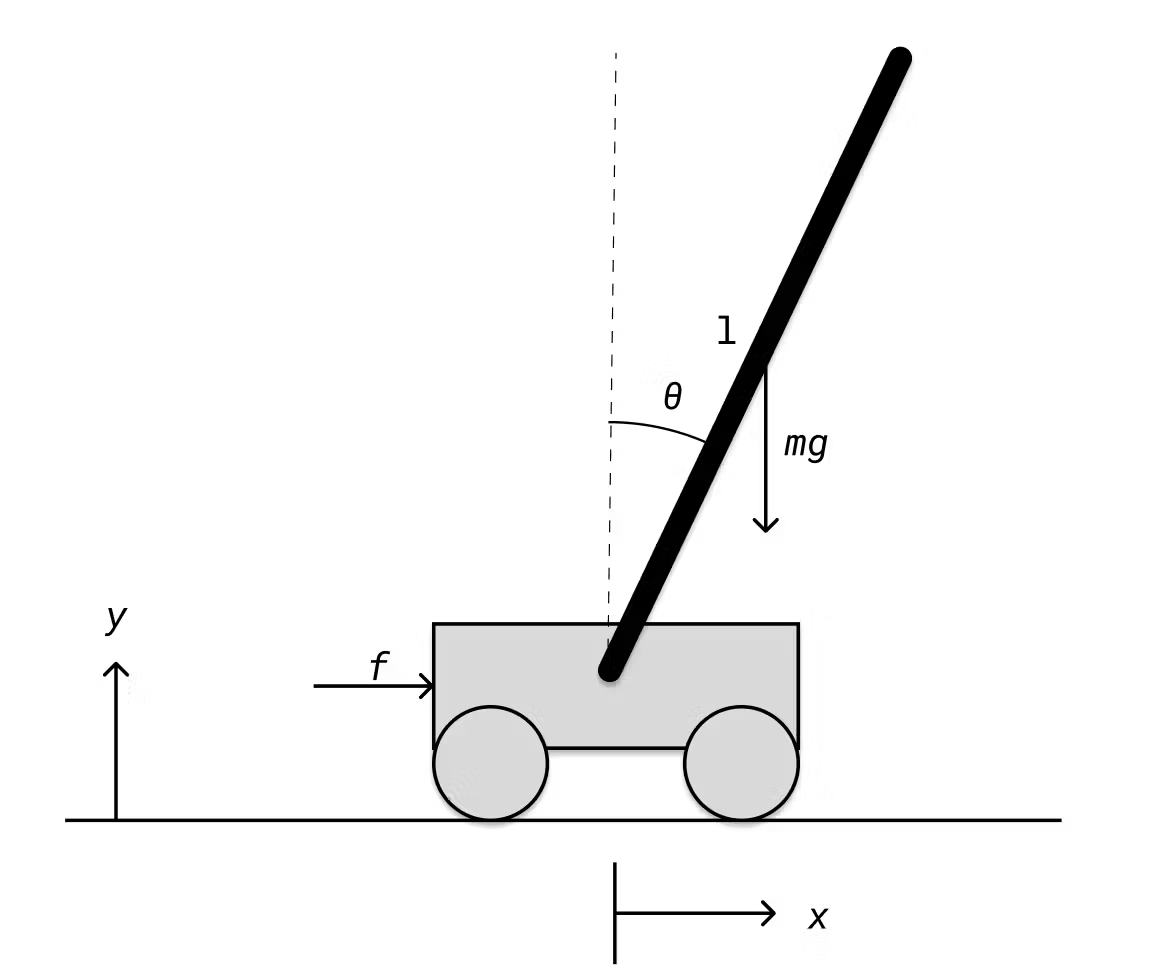
\includegraphics[width=5cm, height=7cm, keepaspectratio]{images/reinforcement_11.png}
\end{center}
\end{column}
\end{columns}
\end{frame}

\begin{frame}[fragile]{Egy egyszerű kezdeti politika}
Az első egy keménykódolt politika: \textbf{olyan statikus szabályrendszer, amelyet nem gépi tanulás segítségével ismer meg az ügynök, hanem egy determinisztikus program vezérli}:
\begin{small}
\begin{center}
\begin{lstlisting}
for episode in range(n_episodes):
	for step in range(n_steps):
		if obs.theta < 0:
			action = 0
		else:
			action = 1
		obs, reward = env.step(action)
\end{lstlisting}
\end{center}
\end{small}
A politika szerint ha a $\theta$ oszlop dőlési szöge kevesebb, mint $0$, a kocsit balra tolja, egyébként jobbra.\par\smallskip
Az \texttt{env.step(action)} függvény segítségével hajtja végre az ügynök a választott cselekvését, majd a környezet visszaadja neki a jutalmat és a következő állapotot. 
\end{frame}

\begin{frame}{Neurális hálózat politika}
\textbf{A szabályok kézzel való implementálása hosszas és túlságosan specifikus.} Ettől egy jobb hozzáállás, ha egy gépi tanulás modell becsüli a cselekvéseket a környezeti változók alapján.\par\smallskip
A modell bemenete ebben az esetben \textbf{a környezeti változók vektora, a kimenete pedig a cselekvés, amit az ügynök végre fog hajtani}. A tanítás eljárása pedig a neurális hálózat javításaként értelmezhető. 
\begin{center}

\includegraphics[width=12cm, height=7cm, keepaspectratio]{graphs/reinforcement_5.png}
\end{center}
\end{frame}

\begin{frame}{Politika hálózat működése}
A hálózat output neuronjai azt a valószínűséget becsülik meg, h\textbf{ogy mekkora valószínűséggel az adott cselekvés lesz a leginkább jövedelmező az ügynök számára}.\par\smallskip
Ezután történik egy véletlen mintavétel, ahol $\varepsilon$ valószínűséggel a legjobb cselekvés fog szerepelni, $1-\varepsilon$ valószínűséggel pedig véletlen cselekvés. \textbf{Ezzel lesz képes az ügynök felfedezni véletlen cselekvéseket a nem várt, de magas jutalom reményében}. 
\begin{center}
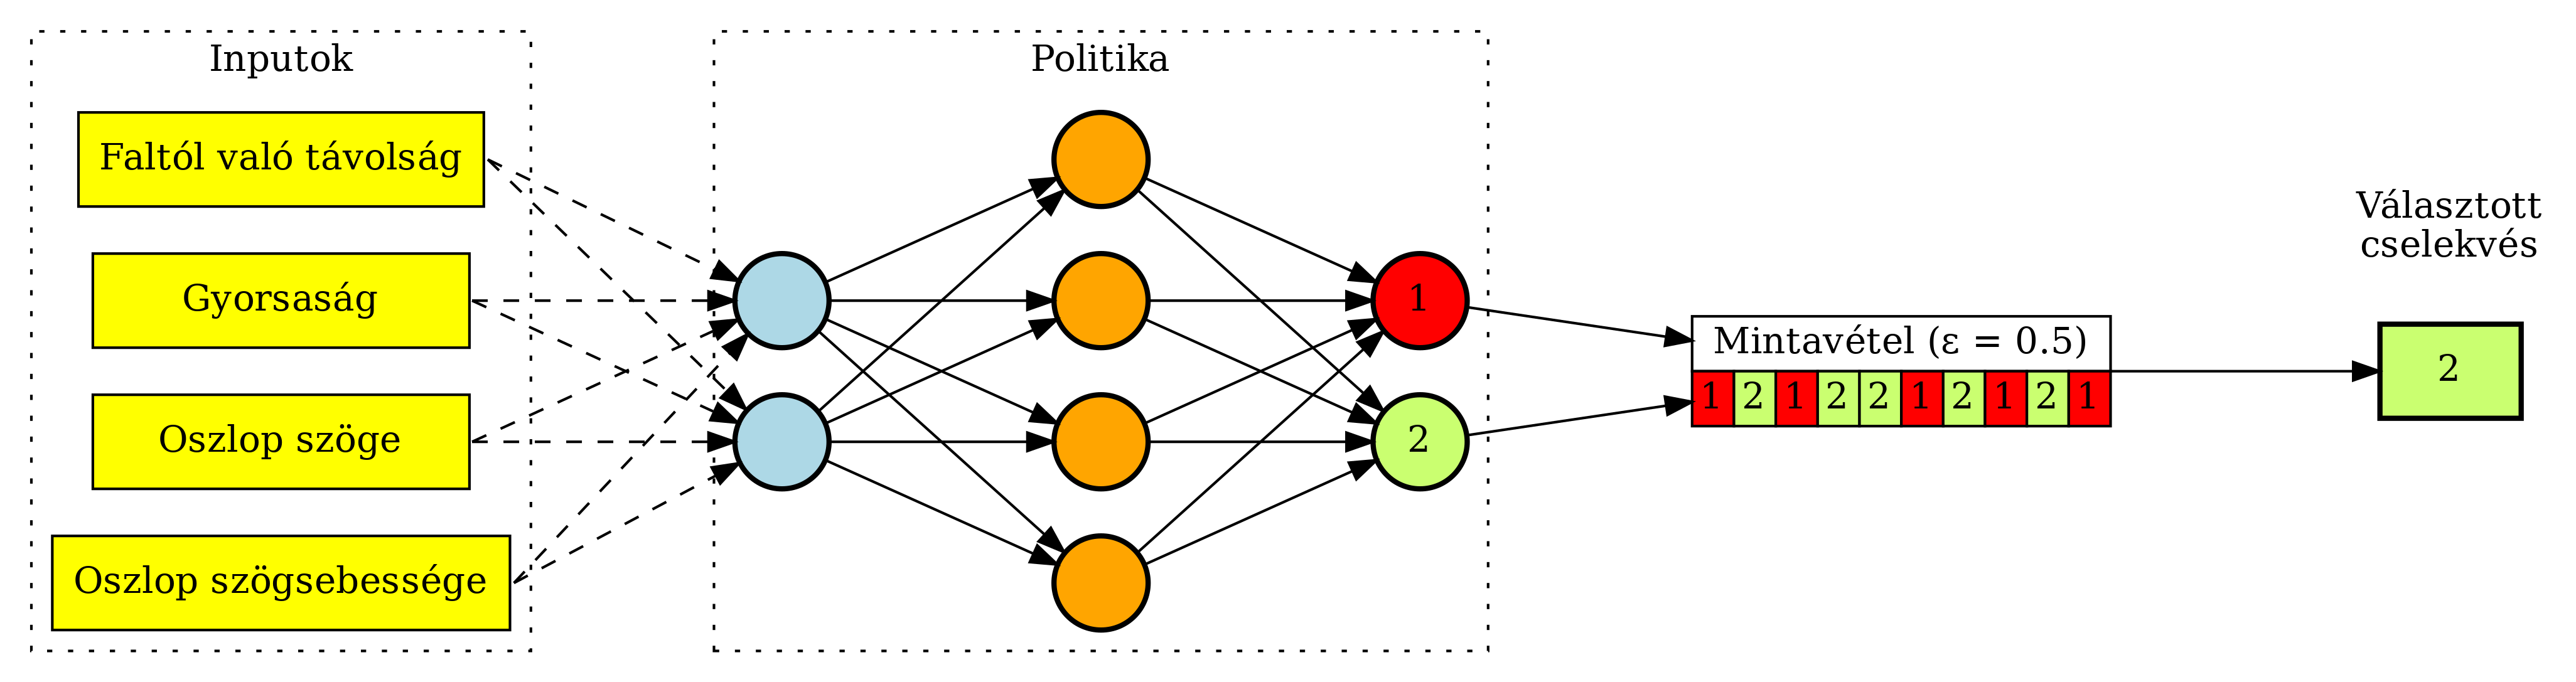
\includegraphics[width=14cm, height=7cm, keepaspectratio]{graphs/reinforcement_6.png}
\end{center}
\end{frame}

\begin{frame}{Tapasztalat visszajátszás}
\begin{columns}
\begin{column}{.5\textwidth}
A tapasztalat visszajátszás a neurális hálózat alapú ügynökök \textbf{belső memóriája}.\par\smallskip
A memória $\left[ s,a,r,s' \right]$ négyeseket tartalmaz. Minden alkalommal amikor az ügynök cselekszik, az általa tapasztalt $s,a,r,s'$ elmentődik.\par\smallskip
A\textbf{mikor tanulási iterációra kerül a sor az ügynök véletlen és rendezetlen mintát kap a visszajátszásból, melynek számossága megegyezik a kötegmérettel}. Eszerint számolja a költségfüggvényt majd frissíti a modell paramétereit. 
\end{column}
\begin{column}{.5\textwidth}
\begin{center}
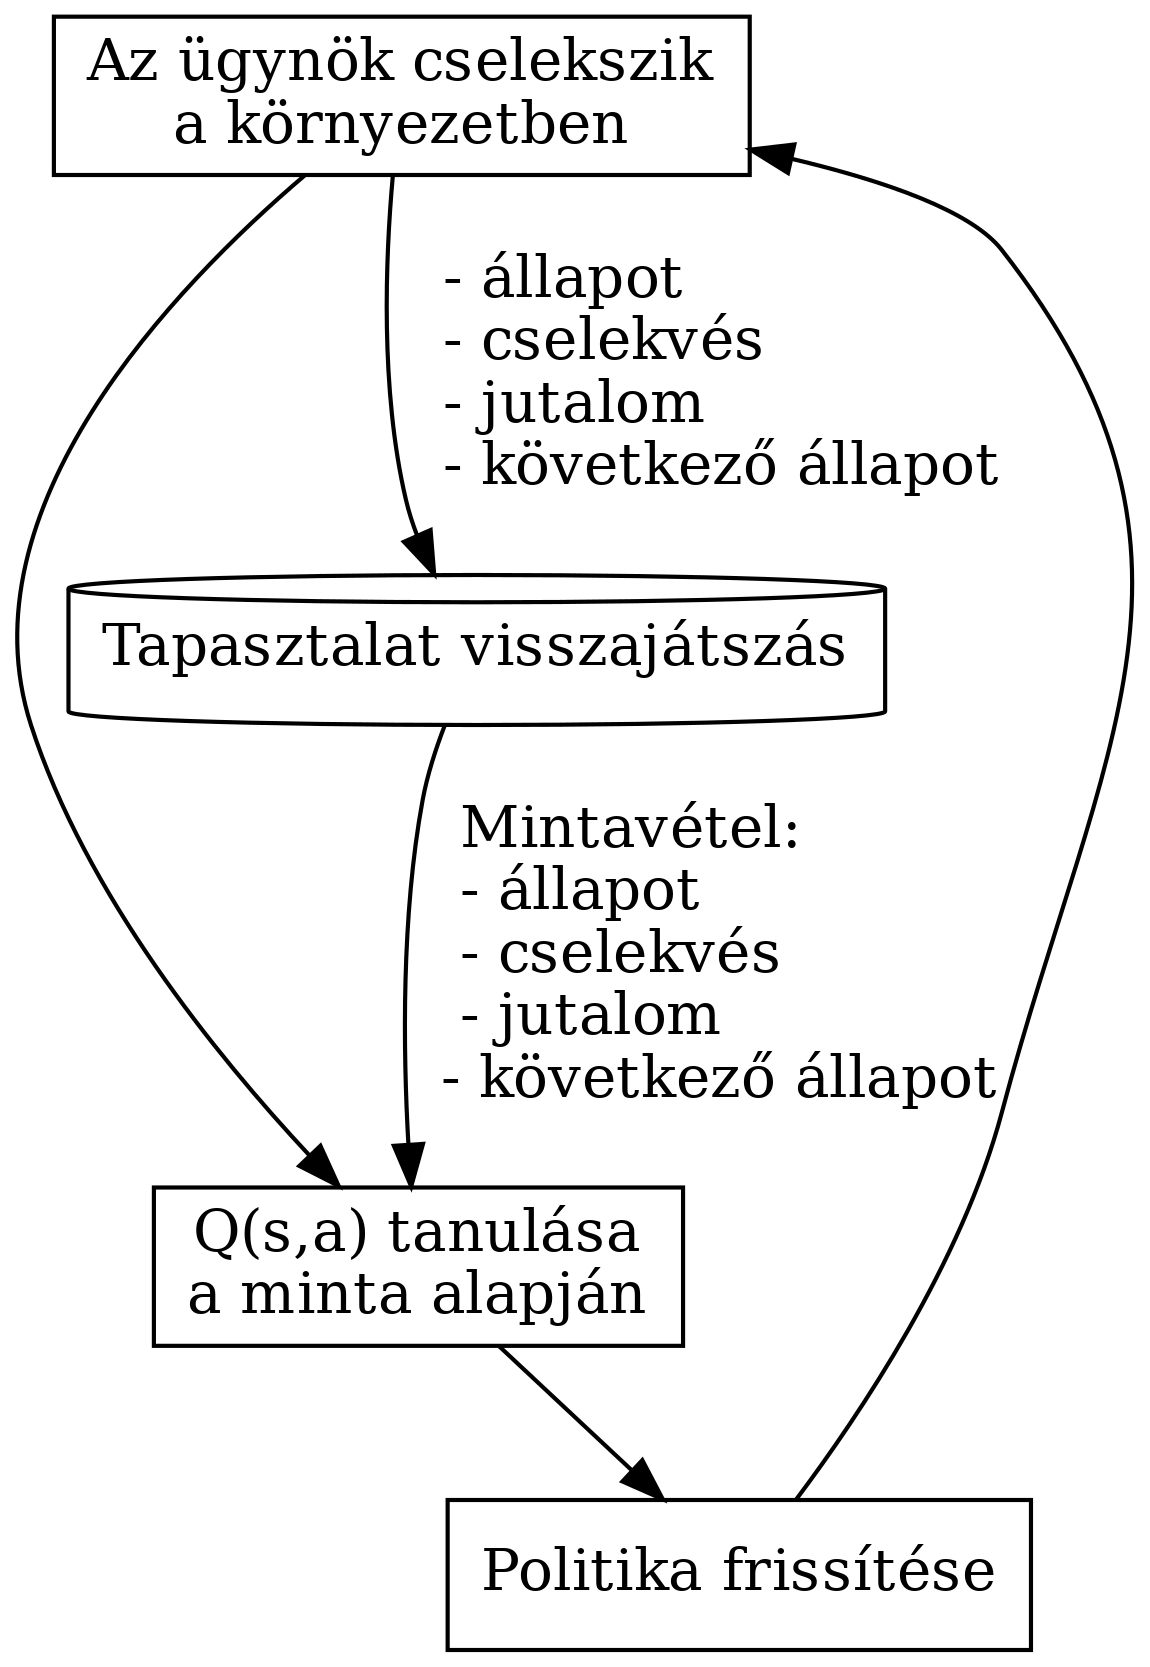
\includegraphics[width=7cm, height=7cm, keepaspectratio]{graphs/reinforcement_9.png}
\end{center}
\end{column}
\end{columns}
\end{frame}

\begin{frame}{A kredit hozzárendelési probléma}
\begin{columns}
\begin{column}{.5\textwidth}
\only<1>{Ha lehetséges lenne tudni minden lépésben, hogy melyik az optimális cselekvés, a neurális hálózat egyszerűen tanítható lenne a keresztentrópia minimalizálásával.\par\smallskip
\textbf{Viszont az RL-ben a visszajelzések ritkák és késleltetettek. Az ügynök egyetlen visszajelzése amit kap, a jutalom, és nem mindig az utolsó cselekvés az, ami felelős a jutalomért.}\par\smallskip
Például: ha az ügynök 100 lépésen keresztül egyensúlyozza a rudat, majd leejti, honnan lehet tudni melyik cselekvés volt a felelős a leejtésért?}
\only<2>{A probléma megoldására az RL bevezet egy $\gamma$ diszkontálási tényezőt, amely \textbf{megadja a jövőbeli jutalmak jelenbeli értékét.} Valamely $r$ jutalom értéke $k$ időlépés után $\gamma^{k-1}$.\par\smallskip
Példa: ha az ágens háromszor jobbra megy, ezután a három jutalma $\left[+10, 0, -50\right]$, és $\gamma=0.8$ az első cselekvés visszatérése $10 + 0 \cdot \gamma + \gamma^2 -50 = -22$.\par\smallskip
\textbf{Ha $\gamma=0$, a modell a jelenbeli jutalmat részesíti előnyben. Ha viszont $1$ közeli az értéke, a hosszú távú jutalomra törekszik.}}
\end{column}
\begin{column}{.5\textwidth}
\begin{center}
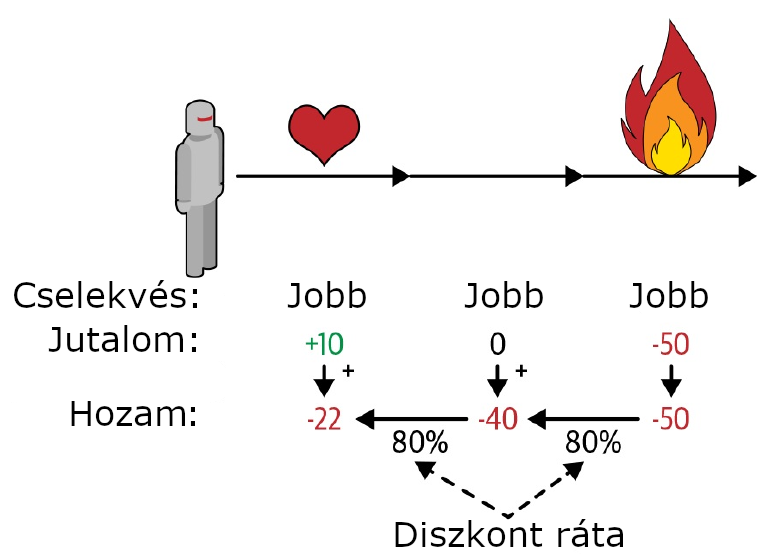
\includegraphics[width=7cm, height=7cm, keepaspectratio]{images/reinforcement_12.png}
\end{center}
\end{column}
\end{columns}
\end{frame}

\begin{frame}{Politika gradiens algoritmusok}
\begin{columns}
\begin{column}{.5\textwidth}
\only<1>{Ahogy a függvényeknek, úgy egy politikának is meghatározható a gradiense.\par\smallskip
A politika gradiens algoritmusok úgy optimalizálják a modellek paramétereit, hogy mindig a magasabb jutalom felé mutató paramétereket növelik.}
\only<2>{A politika gradiens algoritmus magas szintű lépései: 
\begin{enumerate}
	\item Az algoritmus epizódokon keresztül futtatja a politikát.
	\item Miután több epizód lezajlott, az algoritmus kiszámítja mindegyik epizód diszkontált kumulatív jutalmát.
	\item Minden epizódhoz kiszámít egy gradiens vektort, majd megszorozza a hozzá tartozó diszkontált jutalommal.
	\item Az összes, így kapott gradiens vektor átlagolása után az algoritmus egy gradiens ereszkedés lépést hajt végre a politikán.
\end{enumerate}}
\end{column}
\begin{column}{.5\textwidth}
\begin{center}
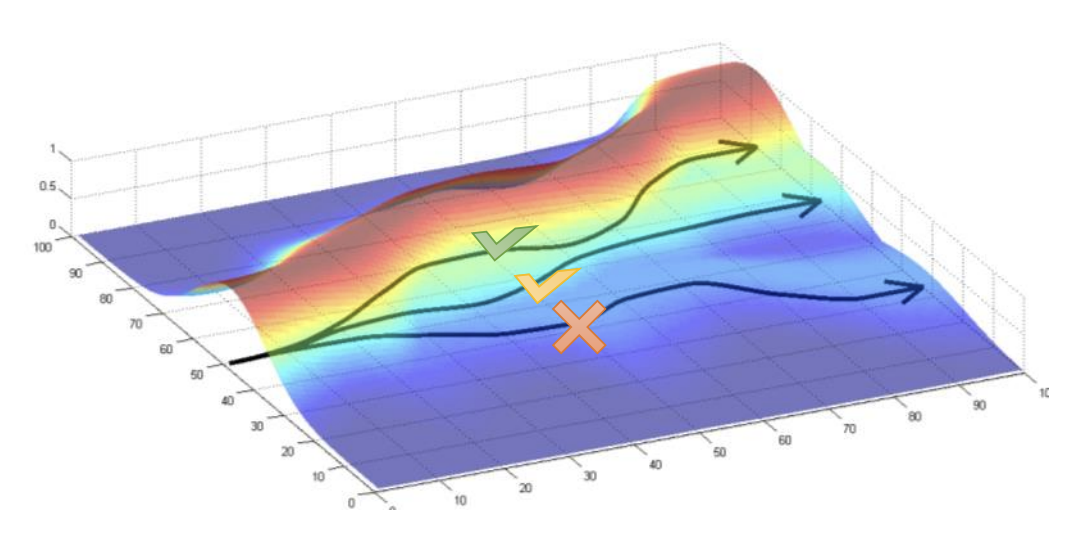
\includegraphics[width=7cm, height=7cm, keepaspectratio]{images/reinforcement_13.png}
\end{center}
\end{column}
\end{columns}
\end{frame}

\section{$Q$-tanulás}

\begin{frame}
\tableofcontents[currentsection]
\end{frame}

\begin{frame}{A $Q$ cselekvés minőség}
\begin{columns}
\begin{column}{.5\textwidth}
\begin{block}{Állapot-cselekvés minőség függvény}
Egy $(s,a)$ állapot-cselekvés páros minőség függvénye valamely $\pi$ politika szerint a várható hozam, \textbf{ha az ügynök $s$ állapotból indul, $a$ cselekvést hajtja végre, majd utána $\pi$ szerint hozza döntéseit}:
\[
Q_{\pi}(s,a)=E_{\pi}\left[G_{t}|S_{t}=s,A_{t}=a\right]=
\]
\[
=E_{\pi}\left[\sum_{k=0}^{\infty}\gamma^{k}r_{t+k+1}\mid S_{t}=s,A_{t}=a\right]
\]
\end{block}
\end{column}
\begin{column}{.5\textwidth}
\begin{center}
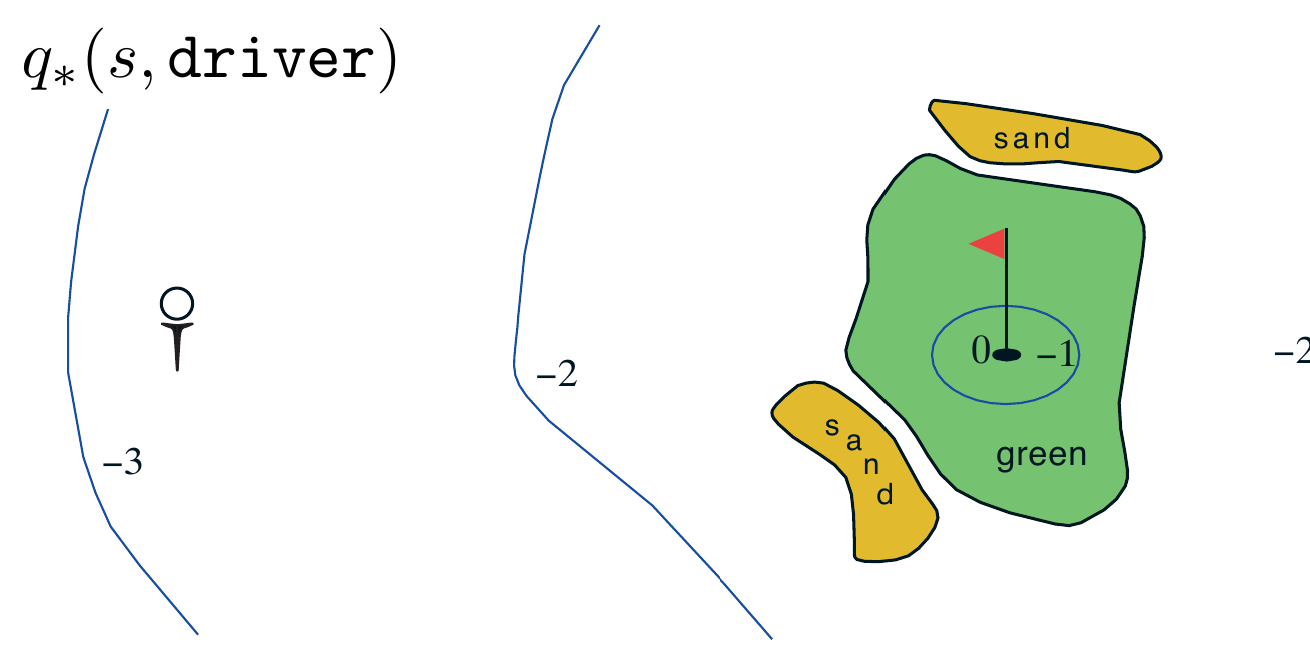
\includegraphics[width=7cm, height=7cm, keepaspectratio]{images/reinforcement_14.png}
\end{center}
\end{column}
\end{columns}
\end{frame}

\begin{frame}{A $Q$-tanulás}
\begin{columns}
\begin{column}{.5\textwidth}
\only<1>{A $Q$-tanulás nem egy politika, hanem egy értékalapú megerősítéses tanulási megközelítés. \textbf{Az értékalapú algoritmusok cselekvések és állapotok értékei alapján határozzák meg a politikát.}\par\medskip
A $Q$-tanulás egy politikafüggetlen tanulási eljárás: az ügynök által végrehajtott politikától függetlenül képes megtalálni az optimális politikához tartozó $Q$-értékeket.}
\only<2>{A $Q$-tanulás általános algoritmusa:
\begin{enumerate}
	\item $Q$-tábla inicializálása véletlen értékekkel
	\item Cselekvés választása a $Q$-tábla alapján
	\item Cselekvés végrehajtása a környezetben 
	\item Jutalom és környezet megfigyelése
	\item $Q$-tábla frissítése
	\item 2-5 lépések ismétlése
\end{enumerate}}
\end{column}
\begin{column}{.5\textwidth}
\begin{center}
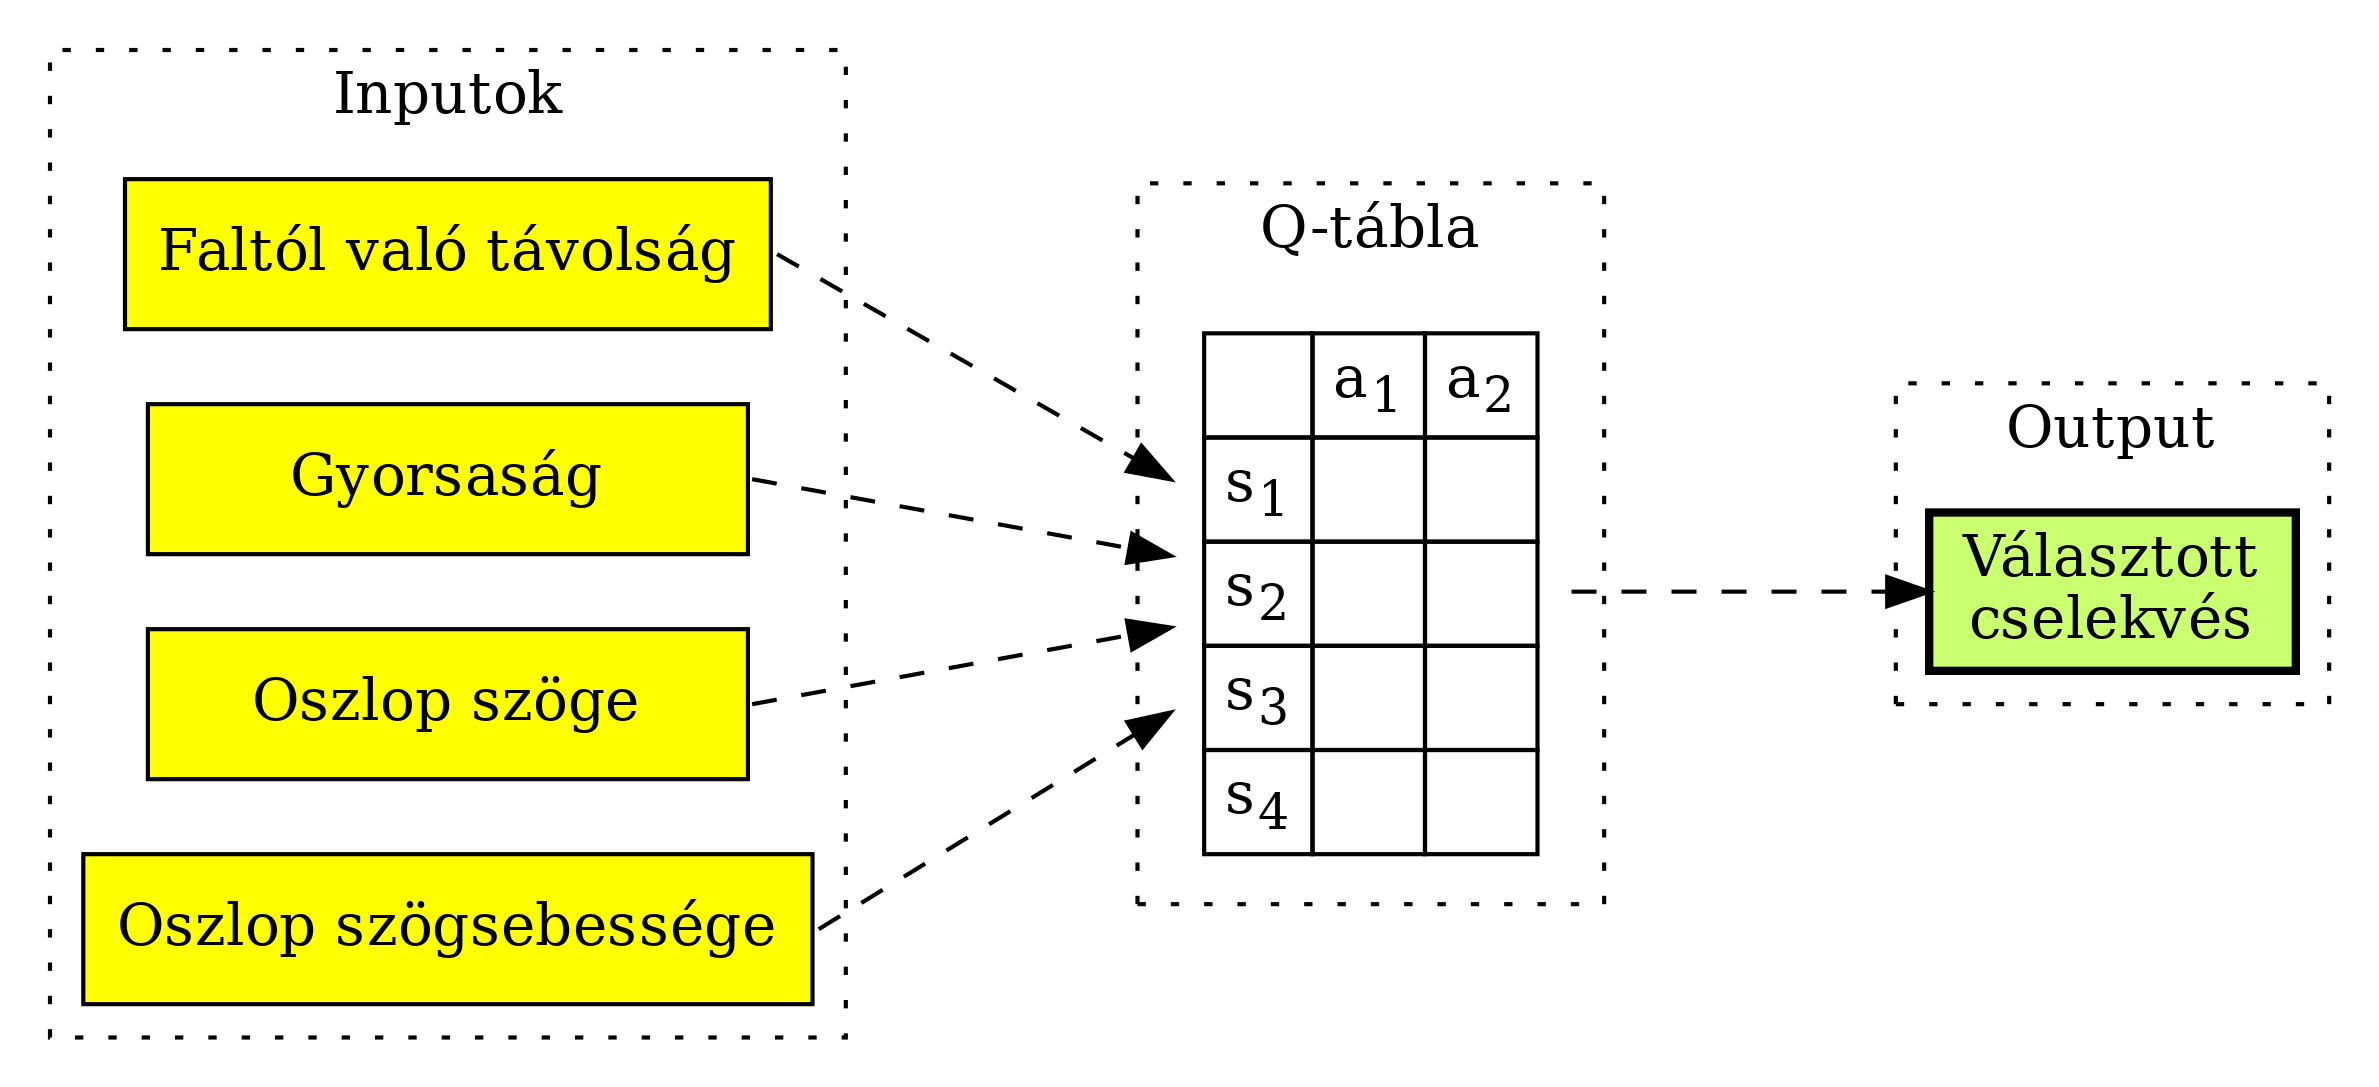
\includegraphics[width=7cm, height=7cm, keepaspectratio]{graphs/reinforcement_7.png}
\end{center}
\end{column}
\end{columns}
\end{frame}

\begin{frame}{$Q$-tábla frissítése}
\begin{columns}
\begin{column}{.65\textwidth}
\begin{block}{$Q$-érték frissítésének szabálya}
\[
Q\left( s,a \right) \leftarrow Q\left( s,a \right) + \alpha \left[ r + \gamma \underset{a'}{max}Q\left( s',a' \right) - Q\left( s,a \right) \right]
\]
Ahol:
\begin{itemize}
	\item $s$: Aktuális állapot
	\item $a$: Aktuális cselekvés
	\item $\alpha$: Tanulási sebesség
	\item $r$: Jutalom 
	\item $\gamma$: Diszkont ráta
	\item $s'$: Következő állapot
	\item $a'$: Következő cselekvés
\end{itemize}
\end{block}
\end{column}
\begin{column}{.35\textwidth}
\begin{footnotesize}
\begin{table}[h]
\centering
Példa $Q$-táblára:\par\medskip
\begin{tabular}{|c||c|c|c|c|}\hline
Állapot & Fel & Le & Bal & Jobb \\\hline
$ s_1 $ & $0.1$ & \textcolor{green}{$0.6$} & $0.2$ & $0.3$ \\\hline
$ s_2 $ & \textcolor{green}{$0.7$} & $0.1$ & $0.4$ & $0.2$ \\\hline
$ s_3 $ & $0.2$ & $0.2$ & \textcolor{green}{$0.8$} & $0.4$ \\\hline
$ s_4 $ & $0.3$ & $0.1$ & $0.5$ & \textcolor{green}{$0.9$} \\\hline
$ s_5 $ & $0.1$ & \textcolor{green}{$0.5$} & $0.4$ & $0.2$ \\\hline
$ s_6 $ & $0.3$ & $0.3$ & \textcolor{green}{$0.6$} & $0.2$ \\\hline
$ s_7 $ & \textcolor{green}{$0.8$} & $0.3$ & $0.1$ & $0.4$ \\\hline
$ s_8 $ & $0.2$ & $0.4$ & $0.3$ & \textcolor{green}{$0.7$} \\\hline
\end{tabular}
\end{table}
\end{footnotesize}
\end{column}
\end{columns}
\end{frame}

\begin{frame}{Cselekvés kiválasztás és végrehajtás}
\begin{columns}
\begin{column}{.5\textwidth}
Mivel az ügynöknek kezdetben nincs ismerete a környezetről, véletlenül kell cselekednie, hogy megismerje mely állapotok és cselekvések milyen jutalommal járnak.\par\smallskip
\begin{block}{$\varepsilon$-mohó cselekvés választás}
\[
a_{t}\leftarrow\begin{cases}
_{a\sim A}^{\underset{a}{argmax}Q_t(a)} & _{P=\varepsilon}^{P=1-\varepsilon}\end{cases}
\]
Ahol $A$ az összes cselekvés halmaza.
\end{block}
\end{column}
\begin{column}{.5\textwidth}
\textbf{Felfedezés}: Véletlen cselekvés végrehajtása, $\varepsilon$ valószínűséggel.\par\medskip
\textbf{Kizsákmányolás}: Már ismert, nagy jutalommal járó cselekvés végrehajtása, $1-\varepsilon$ valószínűséggel. 
\begin{center}
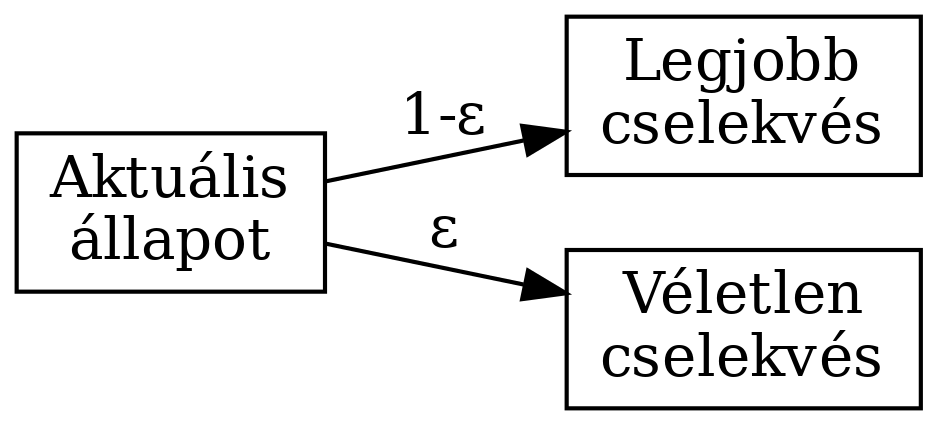
\includegraphics[width=7cm, height=7cm, keepaspectratio]{graphs/reinforcement_8.png}
\end{center}
\end{column}
\end{columns}
\end{frame}

\begin{frame}{Felfedezési stratégia}
\begin{columns}
\begin{column}{.5\textwidth}
Amikor a tanulás folyamata elkezdődik, az ügynöknek fel kell fedeznie a környezetét, és véletlen cselekvések által \textbf{tapasztalatot szereznie}.\par\smallskip
Később, amikor már kellően tapasztalt \textbf{a véletlen cselekvéseket felváltják a legnagyobb értékű cselekvések}. Ennek megfelelően az $\varepsilon$ együttható csökken.\par\smallskip
Az $\varepsilon$ csökkenését a párolgási együttható, $\varepsilon_{decay}$ határozza meg. Minden iterációban a változás:
\[
\varepsilon \leftarrow \varepsilon \cdot \varepsilon_{decay}
\]
\end{column}
\begin{column}{.5\textwidth}
\begin{center}
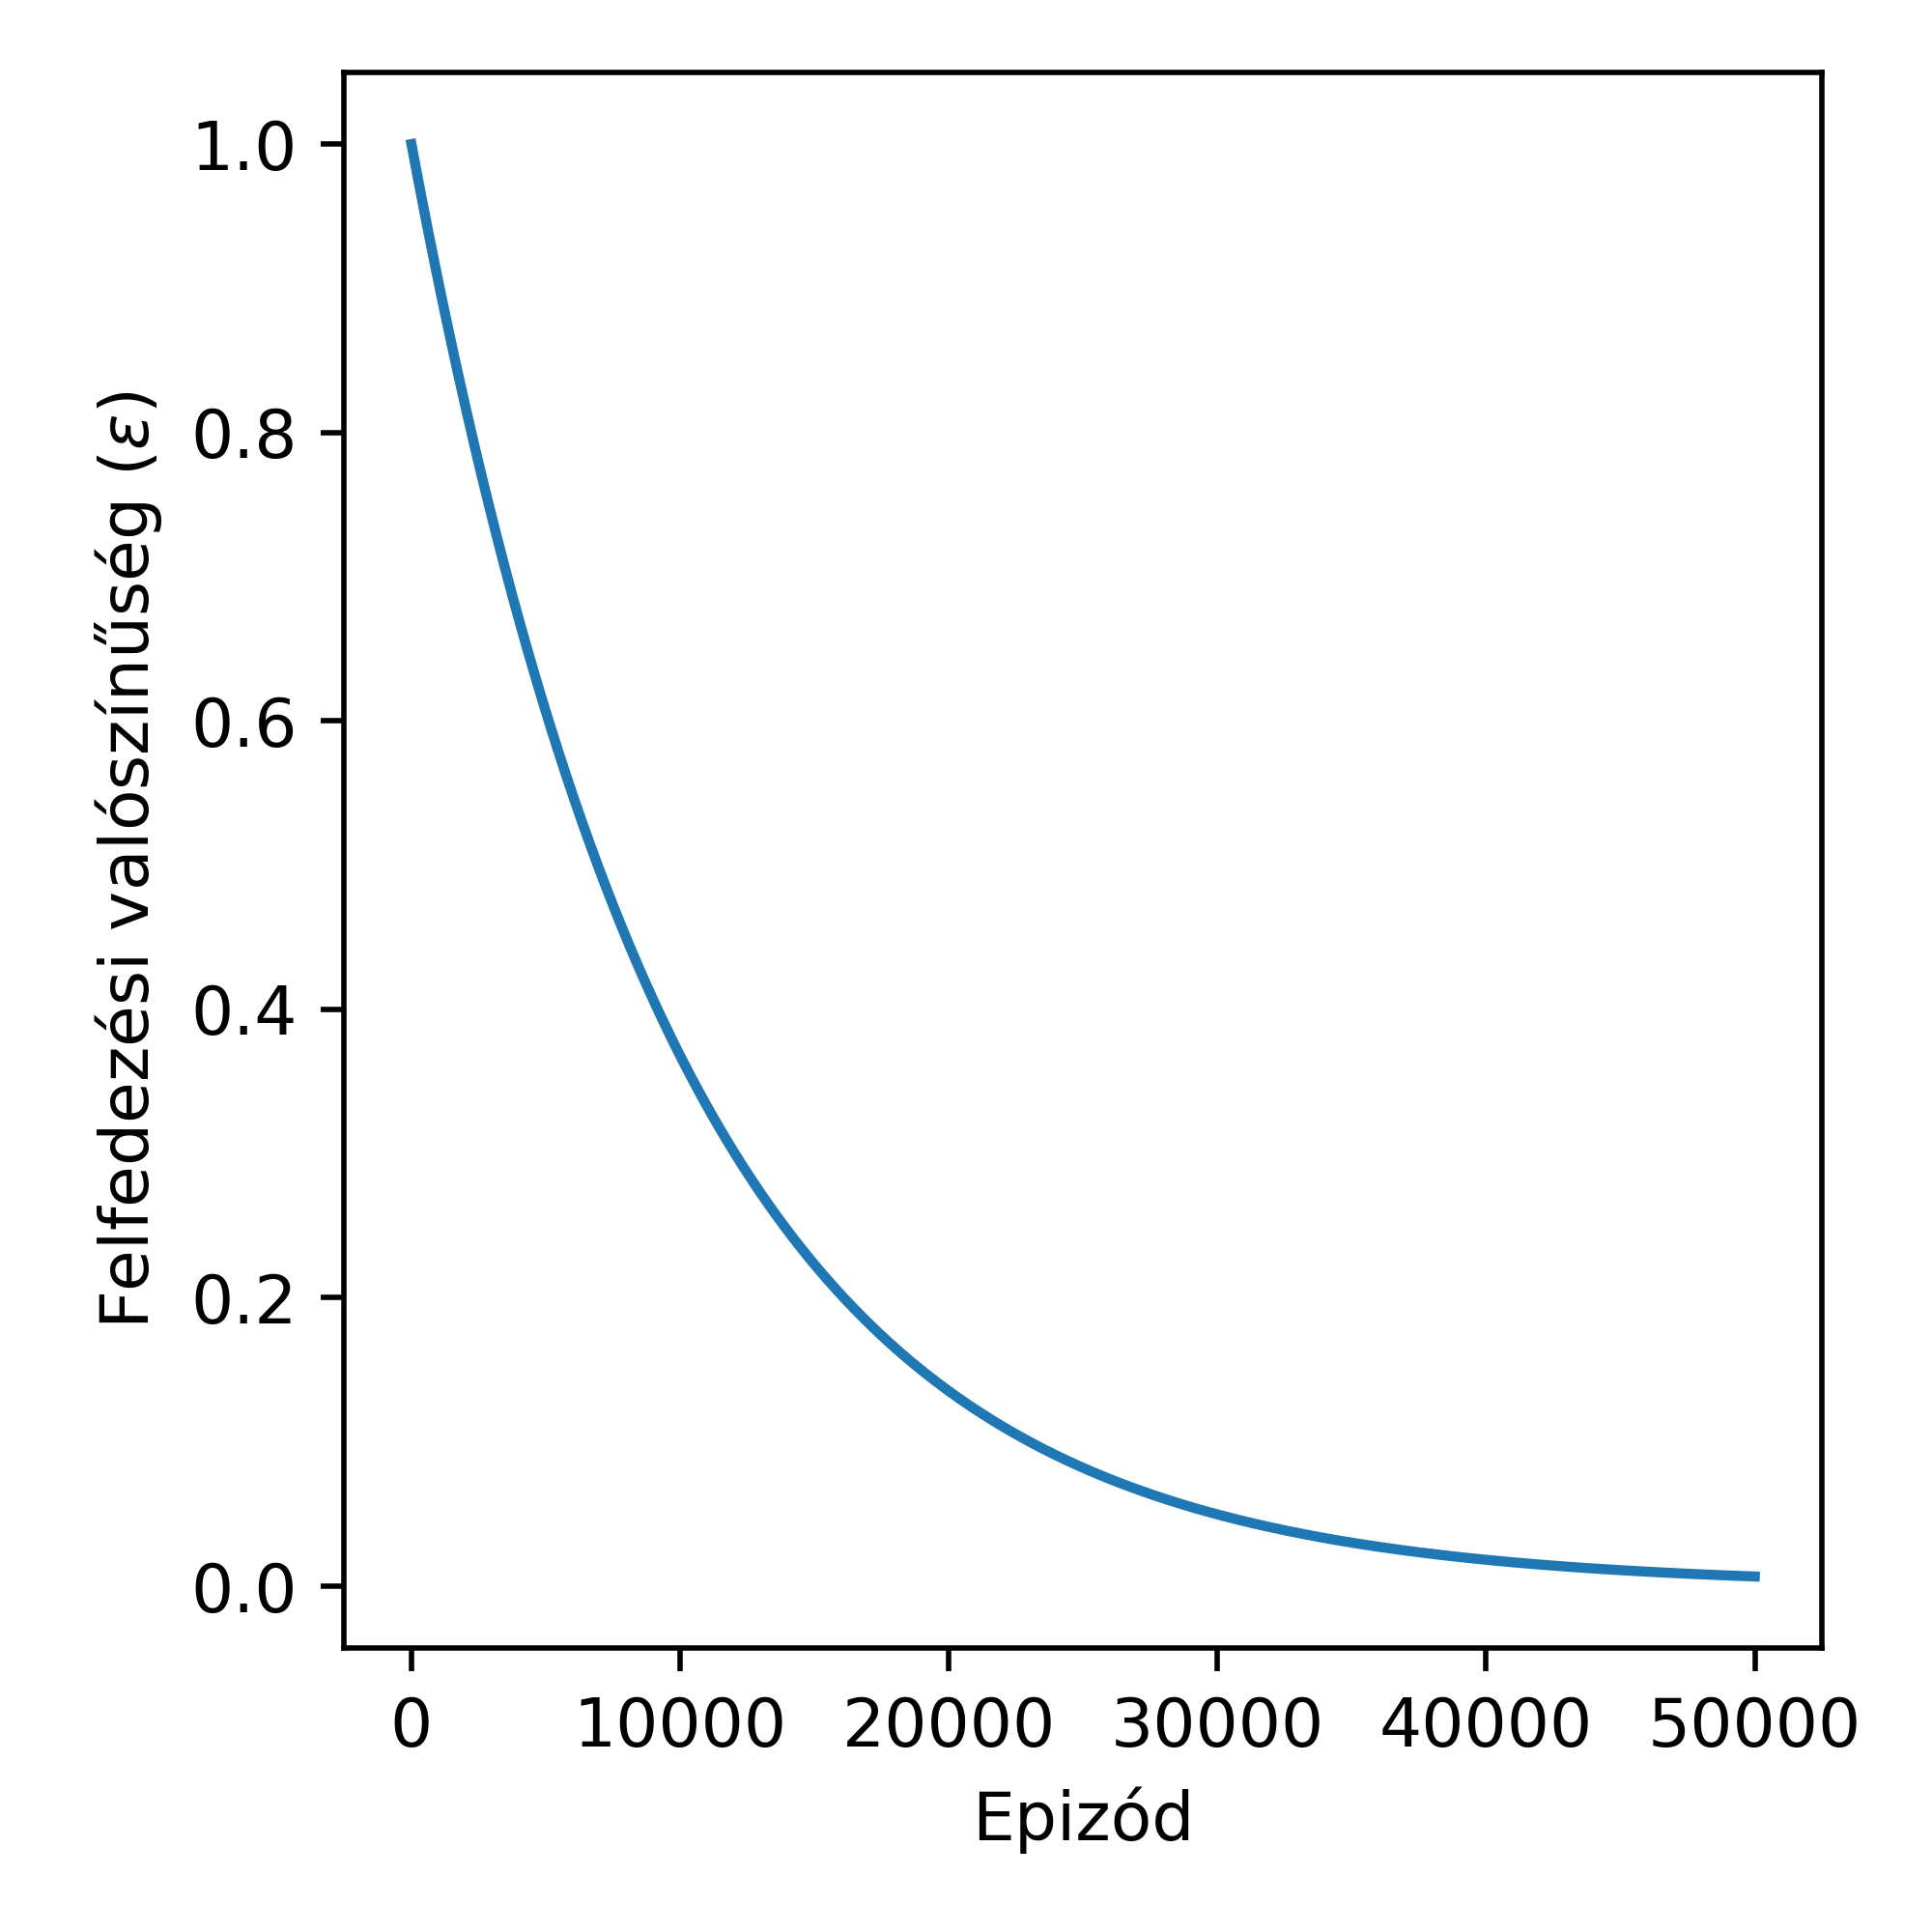
\includegraphics[width=7cm, height=7cm, keepaspectratio]{images/reinforcement_15.png}
\end{center}
\end{column}
\end{columns}
\end{frame}

\end{document}
















